\clearpage

\section{线性方程组}

我们在第一章中看到，
为$\mathbb{K}^n$及其某些子集赋予线性结构，
就从单纯的集合“升级”了向量空间及其线性子空间.
所谓线性结构，
就是指满足封闭性及$8$条运算规则的向量加法和数乘运算.
以此为背景，
我们研究线性方程组，
就不仅是为了得到解集，
更需要留意与解集相关的线性结构.
别忘了，
研究线性方程组就是在研究线性映射.
所以同样的问题也可以表述为：
\textbf{线性映射可以诱导出哪些线性结构？}
我们将通过研究线性方程组回答这一问题.

线性方程组可以用向量组线性表示的观点来看待.
我们在线性代数中谈及向量组，
实际上就是为了讨论它所生成的子空间，
例如谈论矩阵$A$的列向量组就是在谈论$\operatorname{Im}A$.
只要不涉及具体的向量计算，
我们就不需要那几个向量本身的特点.
\textbf{如果两个向量组生成的子空间相同，
我们就称这两个向量组等价}.
从字面意思上理解，
就是说我们只关心各个向量组生成的子空间有什么区别，
而不关心其他的区别.

这一句话已经基本上说清了本章关于向量组的最重要的理解.
其余知识点都是在这句话的基础上雕花——
为什么这么说？
接下来的讨论在讲清楚向量组等价的同时，
也逐步回答这个问题.


\subsection{向量组的等价与向量组的秩}

\subsubsection{向量组的等价}

我们提出了向量组等价的概念：
\textit{两个向量组等价是指它们生成的子空间等价}.
这是从子空间的角度叙述的.
其实这个概念也可以做“翻译”.
按书上的说法：
\textit{两个向量组等价是指它们可以相互线性表示对方的每一个向量.}
为什么这两种说法是同一回事？
以下的命题反映了线性表示下子空间的关系：

\medskip
\textbf{命题2.1.1}~~
\textit{向量组(I)能线性表示向量组(II)的每个向量，
当且仅当(II)生成的子空间是(I)生成的子空间的子集.}
\medskip

得到重要推论：
\textit{两个向量组能相互线性表示，
当且仅当它们生成的子空间互相是对方的子集，
即它们生成的子空间相等.}
\medskip

无论采用哪种说法，
都能轻易得到以下三条性质：

\medskip

\textit{(1)~~（反身性）一个向量组必定与自身等价.}

\textit{(2)~~（对称性）如果向量组(I)与(II)等价，则(II)与(I)也等价.}

\textit{(3)~~（传递性）如果向量组(I)与(II)等价，(II)与(III)等价，
则(I)与(III)等价.}  
\medskip

在今后的学习中，
这三条性质将会绑定在一起，
像咒语一样出现在许多地方.
我们花一些篇幅来解释为什么一定要提这三条性质.
这样之后，
我们就可以更加清楚地用“等价”的语言来讨论问题，
而不只是当作干巴巴的性质来背诵.


\subsubsection{一般意义上的等价关系}

我们在数学中接触过许多“等价”.
例如，我们说两个命题是“等价”的，
意思是两个命题可以相互推出；
我们说两个无穷小量是“等价”的，意思是它们作为独立因式出现在极限式中时可以相互替代.
“等价”这个词究竟是什么意思呢？
粗略地说，
所谓“等价”，
就是说两个事物具有某种共同性质，
以至于在相应的语境中没有必要区分它们，
可以相互替代.
在数学上，
我们可以给“等价”下一个抽象化定义：
\medskip

\textbf{定义（等价关系）}~~
\textit{设$S$是非空集合，“$\sim$”是$S$上的一个二元关系.如果$S$中的两个元素$a$和$b$如果具有该关系，则记作$a \sim b$.
如果“$\sim$”满足以下$3$条性质，
称它是\textbf{$S$的一个等价关系}：
}\hypertarget{equality}{}

\textit{(1)~~（反身性）$a \sim a$.}

\textit{(2)~~（对称性）如果$a \sim b$，则$b \sim a$.}

\textit{(3)~~（传递性）如果$a \sim b$且$b \sim c$，则$a \sim c$.}

\medskip

我们的三条“咒语”就在这里作为等价关系的定义出现了.
因此，
本节开篇的讨论只是验证了向量组的等价的确是一种等价关系.
说它是“向量组等价的$3$条性质”似乎有些本末倒置了，
因为如果没有这$3$条性质，
我们一开始就不会用“等价”这两个字来称呼这种关系.

根据定义，
我们发现许多熟知的关系其实都是等价关系.
例如，实数的相等“$=$”是$\mathbb{R}$的等价关系；
在全体三角形的集合中，
三角形的全等“$\cong$”，
三角形的相似“$\sim$”等等都是不同的等价关系.
在现实生活中，
人的性别相同，血型相同，星座相同等等也都是等价关系.
这些等价关系的验证本身都很显然的.
关键是，
在等价关系的基础上我们能讨论什么更深刻的东西？
\medskip

\textbf{1.~~等价类}

\textit{例1：整数集$\mathbb{Z}$上“除以$2$余数相等”是一个等价关系.
但我们平常对此的理解是：全体整数可以分为奇数和偶数两类.}

\textit{例2：将一个年级中的同学分为若干个班级.
这使得“属于同一个班级”成为该年级同学中的一个等价关系.}
\medskip

以上两个例子表明，
一个等价关系可以看成将集合$S$进行了划分，
相当于对集合中的元素进行“分类”；
而从集合的划分出发，
也可以诱导出“两个元素属于同一类”这一等价关系.
这里的类称为\textbf{等价类}.
简而言之：\textbf{等价关系就是分类.}
为求严谨，
读者可自行验证两个不同的等价类一定没有交集，
符合我们对“分类”的直观理解.

\medskip

\textbf{2.~~代表元}

\textit{例3：只要观察末位数是$0$还是$1$，
就能判断一个整数的奇偶性.}

\textit{例4：在年级大会上给每个班级颁发奖状，
每班派出一名代表上台领奖.}
\medskip

在等价关系中，
相互等价的元素在某种程度上看成是没有区别，可以相互代替的.
在讨论相关问题时，
只要从每个等价类中出一个“代表”，
它就能替代整个等价类中的所有元素.
这称为等价类的\textbf{代表元}.
从每个等价类中选择哪个作为代表元，
原则上是无所谓的，
但是为了自己的方便，
不妨选择形式最简单，特点最鲜明的元素当代表元.
例如，
我们可能会拿$0$和$1$代表偶数和奇数，
而不是$222$和$333$.
班主任派代表上台领奖时，
大概也会请班长上台，
而不是真的随便叫一个人上台.
\medskip


\textbf{3.~~不变量和完全不变量}

\textit{例5：以三角形面积的相等作为等价关系，属于同一个等价类的三角形面积相等.}

\textit{例6：以向量组互相线性表示作为等价关系，
两个向量组等价当且仅当它们生成的子空间相同.
因此，若两个向量组等价，它们生成的子空间维数也相同，
但反之不成立.}
\medskip


我们常说“人以类聚，物以群分”.
具有相同性质的事物会被归为同类，
而归为同类的事物总是具有相同的性质.
这样的性质就能够揭示相应等价关系的本质.

假设对于集合$S$里的每个元素$a$，
我们都能讨论它的某种性质$P(a)$.
在一个等价关系下，
如果每个等价类中所有元素的该性质相同，
称它是该等价关系的\textbf{不变量}.
例如，
生成子空间的维数就是向量组等价的一个不变量.
但是反过来，
如果两个元素的不变量取值相同，
它们也不一定是等价的，
这使我们有些不满意.
最好单凭不变量就能确定等价关系，
即我们希望：两个元素等价当且仅当不变量的取值相同.
这种特殊的不变量称为\textbf{完全不变量}.
只要掌握了一个等价关系的完全不变量，
就可以说对这个等价关系了解得十分通透了.


我们也可以通过直接给出完全不变量的方式来确定一个等价关系.
在例5中，
三角形的面积就是完全的不变量.
这使得例5成为废话文学.
例6就稍有趣些，
它告诉我们\textbf{在向量组的等价中，
向量组生成的子空间就是完全的不变量.
而生成子空间的维数也是不变量，
但不是完全不变量.}
正因如此，
我们可以反过来定义向量组的等价就是指生成的子空间相同，
这使得对于这种等价关系的各种叙述也像例5一样退化为废话文学.
有了这样一些不变量之后，
“向量组互相线性表示”这种不易想象的关系用处就不大了.
本节后续内容就是为这些不变量做注解.

\subsubsection{向量组的秩}

向量组生成子空间的维数是向量组等价的一个不变量.
把它称为\textbf{向量组的秩}，
用rank表示，
即：
$\text{rank}\{ \bm{\alpha}_1 , \bm{\alpha}_2 , \cdots , \bm{\alpha}_s \} = 
\dim \langle \bm{\alpha}_1 , \bm{\alpha}_2 , \cdots , \bm{\alpha}_s \rangle$.
对于矩阵，
也可以研究其列向量组或行向量组的秩.
矩阵的列向量组的秩（即列空间的维数）称为矩阵的\textbf{列秩}，
矩阵的行向量组的秩（即行空间的维数）称为矩阵的\textbf{行秩}.



显然，
如果一个向量组线性无关，
那么它的秩就是向量的个数.
这也是一个向量组所能达到的最大的秩，
因此也称这种向量组是\textbf{满秩}的.
若一个矩阵的列向量组满秩，称这个矩阵是\textbf{列满秩}的；
若一个矩阵的行向量组满秩，称这个矩阵是\textbf{行满秩}的.

如何确定一个向量组的秩？
根据定义，
其实就是要找它所生成的子空间的一组基，
说出它包含多少个向量.
为此，根据基的定义，
我们需要在向量组中找一个“尽可能大的”线性无关的部分组，
使它能线性表示整个向量组里所有的向量.
称这样的部分组是这个向量组的\textbf{极大线性无关组}.
一个向量组可能有多个极大线性无关组，
取法不唯一.
但是在研究秩的时候，
我们不太关心一个向量的极大线性无关组“具体是谁”.
这时就需要向量组等价的概念发挥作用：
\medskip

\textbf{命题2.1.2}
\textit{~~向量组与它的极大线性无关组等价.}

\medskip

\hypertarget{prop5}{}
\textbf{命题2.1.3}
\textit{~~向量组的任意两个极大线性无关组等价.}
\medskip

一个向量组与它的极大线性无关组生成的子空间是完全相同的，
而极大线性无关组恰是这个子空间的一组基.
这样，我们就可以说，
\textit{一个向量组的秩就是它极大线性无关组所含向量的个数}.
这也可以作为向量组的秩的定义.

\subsubsection{极大线性无关组}

本节的知识点到这儿基本结束了.
但是有一个较大的严谨性问题需要解决.
我们来看教材上是如何严格地给极大线性无关组下定义的：\medskip

\textbf{定义（极大线性无关组）}~~
\textit{向量组的一个部分组称为一个极大线性无关组，如果这个部分组本身是线性无关的，但是从向量组的其余向量（如果还有的话）中任取一个添进去，得到的新部分组都线性相关.}\medskip

这个定义同时也暗示了极大线性无关组的构造方法：
在保证部分组线性无关的前提下，
不停地往部分组里添加向量，
直到添不进去了为止.
但这也引出了一个问题：
\textbf{极大线性无关组所含向量的个数是唯一的吗？}
从同一个向量组的不同向量出发，分别构造极大线性无关组，
它们的向量个数是否可能不一样？
如果这种情况发生，
我们刚才对于秩的定义就不成立了.
另一方面，
说“秩是向量组生成子空间的维数”，
也面临着同样的问题：
仿照极大线性无关组的构造方法，
从子空间中任意一个非零向量出发，
都可以扩展成这个子空间的一组基，
那么基所包含的向量个数是否可能不一样？
这个疑问会动摇“维数”这一概念的合理性.

你可能会反驳：“
所谓‘极大线性无关组’，
难道不就是保证线性无关的‘最大’的部分组吗？
而‘最大值’当然是唯一的了.”
这句话本身是没错的.
但是极大线性无关组的定义并不能直接告诉我们这一点.
在给出数学证明之前，
当然可以怀疑“如果从不同的向量出发来构造极大线性无关组，
构造出来的向量个数也许是不一样的”，
这好比一个函数在不同的地方可能有不同的极大值，
而极大值不一定是最大值.

为了修复上述的bug，
我们要证明\textbf{向量组的任意两个极大线性无关组所含向量的个数相等}，
从而可以将这个数定义为向量组的秩.
由上一小节的\hyperlink{prop5}{命题2.1.3}，
只需要证明等价的线性无关向量组的向量个数一定相同.
这过程非常简短.
先证明关键引理：

\medskip
\textbf{引理2.1.4}
\textit{~~如果向量组(II)能被(I)线性表示，
而(II)的向量个数比(I)还多，
那么(II)是线性相关的.}

\textbf{证明\ } (II)生成的子空间$V_2$是(I)生成的子空间$V_1$的子集
$\Longrightarrow$
$\dim V_2 \le \dim V_1$
$\Longrightarrow$
(II)的极大线性无关组的向量个数$\le$
(I)的极大线性无关组的向量个数
$<$
(I)的向量个数
$<$
(II)的向量个数
$\Longrightarrow$
(II)线性相关.\medskip

如果两个线性无关的向量组等价，
而它们的向量个数不同的话，
根据引理2.1.4，
其中必有一个向量组是线性相关的，矛盾.
因此有：


\medskip

\textbf{命题2.1.5}
\textit{~~两个等价的线性无关的向量组，向量个数一定相同.}\medskip


这样就完成了证明.
现在，我们可以自信地说“向量组的秩就是极大线性无关组的向量个数”了.
但也不要忘记我们一开始对秩的定位：
\textbf{向量组的秩就是它生成的子空间的维数.}
还不要忘记\textbf{向量组的秩和向量组生成的子空间都是向量组等价的不变量.}
书上的以下命题都是它们的自然推论（完全可以通过子空间的叙述简短地完成证明）：

\medskip

\textbf{命题2.1.6}
\textit{~~如果向量组(I)能被(II)线性表示，
则前者的秩不超过后者.}

\textbf{证明\ }
向量组(I)能被(II)线性表示
$\Longrightarrow$
(I)生成的子空间$V_1$是(II)生成的子空间$V_2$的子集
$\Longrightarrow$
$\dim V_1 \le \dim V_2$.
$\Longleftrightarrow$
$\text{rank}(\mathrm{I}) \le \text{rank}(\mathrm{II})$.

\medskip

\textbf{命题2.1.7}
\textit{~~如果两个向量组的秩相等，且其中一个可被另一个线性表示，则它们等价.}

\textbf{证明\ }
设向量组(I)能被(II)线性表示
$\Longleftrightarrow$
则(I)生成的子空间$V_1$是(II)生成的子空间$V_2$的子集
$\Longleftrightarrow$
$V_1$的任意一组基是$V_2$的子集
$\Longrightarrow$
$V_1$的任意一组基也是$V_2$的一组基（因为(I)与(II)的秩相等）
$\Longleftrightarrow$
$V_1 = V_2$
$\Longleftrightarrow$
向量组(I)与(II)等价.\medskip

上文中用子空间的思路简单写了两个命题的证明，
意在展示子空间对于研究向量组的作用.
这也是教材知识所允许的证法.
教材中受到讲解顺序的限制，
只能采用线性表示、线性方程组的观点来证明，
也可以参考学习.
本小节涉及的计算题，
主要是计算向量组的极大线性无关组.
计算向量组的秩，
以及判断两个向量组是否等价.
解决此类问题的好方法在后文讲述
（见2.2.1和2.3.1小节）.


\subsection{线性方程组的解}

\subsubsection{线性方程组解的判别准则}

之前从线性表示和子空间的角度简述过如果判断线性方程组是否有解，
有唯一解还是无穷解\hyperlink{jie}{（传送门）}.
现在有了秩的概念，
我们可以完全改为用秩的方式来叙述.
这有一定的实际意义，
因为计算秩比计算子空间更方便，
前者更适合作为判别工具.\medskip


在本章以后的部分中，
默认线性方程组的形式为：
\begin{eq1}
    x_1 \bm{\alpha}_1 
    + x_2 \bm{\alpha}_2
    + \cdots 
    + x_n \bm{\alpha}_n 
    =
    \bm{\beta} 
    ~~~~
    \textbf{或}
    ~~~~
    A \bm{x} = \bm{\beta}   \end{eq1}

其中，$\bm{\alpha}_i,~\bm{\beta} \in \mathbb{K}^m,~i=1,2,\cdots,n$.
系数矩阵$A = (\bm{\alpha}_1 ,~ \bm{\alpha}_2 , \cdots , \bm{\alpha}_n)$是$m \times n$矩阵.
把系数矩阵与常数列向量$\bm{\beta}$拼在一起成为一个矩阵$\tilde{A} = (A,\bm{\beta})$，
称为线性方程组的\textbf{增广矩阵}.
增广矩阵可以看成线性方程组省略所有运算符号和未知量的偷懒写法.
适合这个方程的$n$维数组$\bm{x}$是$\mathbb{K}^n$中的元素，
称为方程的\textbf{解向量}.

\medskip

\textbf{定理2.2.1（线性方程组有解判别定理）}
\textit{~~线性方程组有解的充要条件是它的系数矩阵$A$
与增广矩阵$(A,\bm{\beta})$的列秩相同.}

\textbf{证明\ }
线性方程组有解
$\Longleftrightarrow$
$A$的列向量组能线性表示$\bm{\beta}$
$\Longleftrightarrow$
$\bm{\beta} \in \operatorname{Im}A$
$\Longleftrightarrow$
$\operatorname{Im}A=\operatorname{Im}(A , \bm{\beta})$
$\Longleftrightarrow$
$A$与$(A , \bm{\beta})$的列秩相同.
（最后一步的等价需考虑到$\operatorname{Im}A$与$\operatorname{Im}(A,\bm{\beta})$有包含关系.）
\medskip

\textbf{命题2.2.2}
\textit{~~当线性方程组有解时，它有唯一解的充要条件是$A$列满秩.}

\textbf{证明\ }已知$\bm{\beta}$能被$A$的列向量组线性表示，
则线性方程组有唯一解
$\Longleftrightarrow$
表示方法唯一
$\Longleftrightarrow$
$A$的列向量组线性无关
$\Longleftrightarrow$
$A$列满秩.\medskip

\textbf{命题2.2.3}
\textit{~~当线性方程组有解时，
它有无穷多解的充要条件是$A$不是列满秩.}

\textbf{证明\ }由(2)的逆否命题立即得到.\medskip

借助这个定理，
我们有简单的方法可以判断两个向量组是否等价.\medskip

\textbf{命题2.2.4}
\textit{~~对于两个行数相同的矩阵$A$和$B$，
$A$和$B$的列向量组等价当且仅当$A,~B$和$(A,B)$的列秩都相同.}

\textbf{证明\ }
将$B$的列向量逐个添加进$A$的列向量组中，秩总是不变，就表明$A$的列向量组能线性表示$B$的每一个列向量.

将$A$的列向量逐个添加进$B$的列向量组中，秩总是不变，就表明$B$的列向量组能线性表示$A$的每一个列向量.

\subsubsection{线性方程组的等价与初等变换}

讲到目前为止，
我们至少还面对着两个实际应用层面的问题:
第一，如何求出向量组的秩和极大线性无关组；
第二，仅使用秩的概念，
只能判断出线性方程组解集的大小，
不足以告诉我们解集具体是谁.
这要求我们依据现有的理论，
发展出一套具体的算法.

我们曾在第一章提到过解线性方程组的问题——
这似乎连小学生都会做.
考虑解以下二元一次方程组的过程:
\begin{eq1}
    \begin{cases}
        2x + y = 2 \\[2pt]
        5x + 5y = 5
    \end{cases}
    \sim ~
    \begin{cases}
        5x + 5y = 5  \\[2pt]
        2x + y = 2 
    \end{cases}
    \sim ~
    \begin{cases}
        2x + 2y = 2  \\[2pt]
        2x + y = 2 
    \end{cases}
    \sim ~
    \begin{cases}
        2x + 2y = 2  \\[2pt]
        0x - y = 0 
    \end{cases}
    \sim ~
    \begin{cases}
        x = 1  \\[2pt]
        y = 0 
    \end{cases} \end{eq1}

对解方程的过程进行总结，
其实无非是反复进行以下三类基本操作，
达到消元化简的目的：\medskip

\textit{(i)~~交换某两条方程的顺序}

\textit{(ii)~~将某条方程整体乘以一个非零系数$k$}

\textit{(iii)~~将某条方程的$k$倍加到另一条方程上} \medskip

这三类基本操作统称为线性方程组的\textbf{初等变换}，
也是我们从小接触的线性方程组的算法.
初学解方程的小朋友可能会问：
为什么这三种操作一定是对的？
设想他得到了两种风格迥异的回答.
一个人没好气地说：
“初等变换这么简单的东西还用说吗？
方程的顺序交换交换有什么区别？
整条方程乘以同一个数不是跟没乘一样吗？”
另一个人耐心地解释说：
“假如一组$(x,y)$是原来那个方程的解，
那么方程经过初等变换之后它仍然是解；
如果不是原方程的解，那么初等变换之后仍然不是.”
后一个人其实是在说\textbf{初等变换保持线性方程组的解集不变}.
而前一个人并非不知道这一点.
恰恰相反，
他对这一点知道得太深，
以至于觉得方程组经初等变换前后是“没区别”的.
这种想法的背后就隐藏了一个等价关系.
我们把它摆到台面上说清楚：\medskip

\textbf{定义（线性方程组的等价）}~~
\textit{如果两个线性方程组可以通过初等变换相互转化，称这两个线性方程组等价.}\medskip

容易验证线性方程组的等价满足反身性、对称性和传递性，
因此它确实是一个一般意义上的
\hyperlink{equality}{\textbf{等价关系}}.
线性方程组的解集就是这个等价关系的不变量，
而且是完全不变量.
所谓解线性方程组，
就是找到与该方程组同属一个等价类的某种异常简单的代表元（注意这里的“代表元”也是一个线性方程组）.
这个代表元能让人一眼看出它的解集.
在上面的例子中，
最末一个方程组$x=1,y=0$就是这样的代表元，
这个线性方程组简单到我都不想称它为线性方程组.
\medskip

增广矩阵是对线性方程组的简记.
可以用增广矩阵的形式来表达上述线性方程组的初等变换（增广矩阵中的虚线只是方便分清系数和常数项）：
\begin{eq1}
        \left ( \begin{array}{cc:c}
             2 & 1 & 2 \\[2pt]
             5 & 5 & 5 \\
        \end{array} \right )
        \overset{r}{\sim}
        \left ( \begin{array}{cc:c}
             5 & 5 & 5 \\[2pt]
             2 & 1 & 2 \\
        \end{array} \right )
        \overset{r}{\sim}
        \left ( \begin{array}{cc:c}
             2 & 2 & 2 \\[2pt]
             2 & 1 & 2 \\
        \end{array} \right )
        \overset{r}{\sim}
        \left ( \begin{array}{cc:c}
             2 & 2 & 2 \\[2pt]
             0 & -1 & 0 \\
        \end{array} \right )
        \overset{r}{\sim}
        \left ( \begin{array}{cc:c}
             1 & 0 & 1 \\[2pt]
             0 & 1 & 0 \\
        \end{array} \right )
        \end{eq1}

可见线性方程组的初等变换就是对增广矩阵的行做变换.
相应的三种基本操作是：\medskip

\textit{(i)~~交换某两行的顺序}

\textit{(ii)~~将某一行乘以一个非零系数$k$}

\textit{(iii)~~将某一行的$k$倍加到另一行上} \medskip

对于矩阵的这三类基本操作，
统称为矩阵的\textbf{初等行变换}.
这也定义了矩阵之间的一种等价关系：
\textit{如果两个矩阵可以通过初等行变换相互转化，称这两个矩阵是行等价的，用符号“$\overset{r}{\sim}$”表示}.
显然，
把矩阵看作线性方程组的增广矩阵时，
矩阵行等价的不变量就是线性方程组的解集.

将来对矩阵的行等价（初等行变换）会有更深刻的讨论.
先讨论它最直接的应用：解线性方程组.

\subsubsection{简化行阶梯形矩阵}

为了解线性方程组，
需要利用初等变换（初等行变换），
把线性方程组（增广矩阵）化成一种最简的形状.
那该是什么样的形状呢？
通过刚才的例子，
你可能已经想到了如下的形状：
\begin{eq1}
        \left ( \begin{array}{cccc:c}
            1 & * & * & * & * \\[2pt]
            0 & 1 & * & * & * \\[2pt]
            0 & 0 & 1 & * & * \\[2pt]
            0 & 0 & 0 & 1 & * \\
        \end{array} \right )
        ~~ 
        \text{或者}
        ~~
        \left ( \begin{array}{cccc:c}
            1 & 0 & 0 & 0 & * \\[2pt]
            0 & 1 & 0 & 0 & * \\[2pt]
            0 & 0 & 1 & 0 & * \\[2pt]
            0 & 0 & 0 & 1 & * \\
        \end{array} \right )
        \end{eq1}


    补充说明：我认为在矩阵中用大量省略号不便于观察形状，
    所以就默认以$4 \times 5$的增广矩阵为例来展示.
    其余尺寸的矩阵可自行类比. 
    矩阵中的星号“*”代表该位置可以是$0$也可以是非零元.
    每一行的第一个非零元称为\textbf{主元}.
    我干脆把主元都记作$1$.
    这是因为当主元不是$1$时，
    我们总能通过把这一行乘以主元的倒数，
    使主元变成$1$.
\medskip

在上面展示的两种增广矩阵的形状中，
后者当然是最最简单的形状，
不过前者也已经够用.
因为第四行直接显示了$x_4$的值.
代入倒数第二行又能立即解出$x_3$.
就这样逐行从下往上代入，
就解出了所有未知量.

现在的问题是，
这两种形状只能代表线性方程组有唯一解的情形.
如果是无解或者有无穷多解，
又该化成什么形状？

只需要考虑具体的化简过程.
假设初始状态下，
增广矩阵左上角的元素不是$0$.
那么可以通过把第$1$行乘以$k$倍加到其他行上，
把第$1$列的其他元素都消成$0$：
\begin{eq1}
    \left ( \begin{array}{cccc:c}
            1 & * & * & * & * \\[2pt]
            * & * & * & * & * \\[2pt]
            * & * & * & * & * \\[2pt]
            * & * & * & * & * \\
        \end{array} \right )
        ~~\to~~
        \left ( \begin{array}{cccc:c}
            1 & * & * & * & * \\[2pt]
            0 & * & * & * & * \\[2pt]
            0 & * & * & * & * \\[2pt]
            0 & * & * & * & * \\
        \end{array} \right )
        \end{eq1}

第$1$列处理完毕，
来看第$2$列.
首先找到第$2$列的一个主元——
当然，有一种可能性是第$2$列根本找不到主元了，
即：
\begin{eq1}
    \left ( \begin{array}{cccc:c}
            1 & * & * & * & * \\[2pt]
            0 & 0 & * & * & * \\[2pt]
            0 & 0 & * & * & * \\[2pt]
            0 & 0 & * & * & * \\
        \end{array} \right )
        \end{eq1}

这样的话我们就可以快乐地跳过第$2$列去看第$3$列了.
如果不是这种情况，
我们适当地交换行的顺序，
使第$2$行的主元处在第$2$列：
\begin{eq1}
    \left ( \begin{array}{cccc:c}
            1 & * & * & * & * \\[2pt]
            0 & 1 & * & * & * \\[2pt]
            0 & * & * & * & * \\[2pt]
            0 & * & * & * & * \\
        \end{array} \right )
        \end{eq1}

仿照刚才的做法继续我们的消消乐.
此时你有两种做法.
如果你只想化简到“够用就行”，
只需要把主元下方的元素都消成$0$；
如果你想追求最最简单的形式，
那么需要把主元所在列的所有其他元素都消成$0$.
分别得到如下的形状：
\begin{eq1}
    \left ( \begin{array}{cccc:c}
            1 & * & * & * & * \\[2pt]
            0 & 1 & * & * & * \\[2pt]
            0 & 0 & * & * & * \\[2pt]
            0 & 0 & * & * & * \\
        \end{array} \right )
        ~~ 
        \text{或者}
        ~~
        \left ( \begin{array}{cccc:c}
            1 & 0 & * & * & * \\[2pt]
            0 & 1 & * & * & * \\[2pt]
            0 & 0 & * & * & * \\[2pt]
            0 & 0 & * & * & * \\
        \end{array} \right )
        \end{eq1}

如此，依次处理每个列，
直到处理完增广矩阵的最后一个列.
如果你是以“够用就行”为目标化简的，
化简完毕的结果有一个显著的特征，
那就是以主元为分界线，
矩阵的左下半区全都是$0$，
形状类似于楼梯.
因此，
将这种形状的矩阵称为\textbf{行阶梯形矩阵}.
以下几种形状的矩阵都是行阶梯形矩阵：
\begin{eq1}
    \text{(I):}
    \left ( \begin{array}{cccc:c}
            1 & * & * & * & * \\[2pt]
            0 & 1 & * & * & * \\[2pt]
            0 & 0 & 1 & * & * \\[2pt]
            0 & 0 & 0 & 1 & * \\
        \end{array} \right )
        ~~~~~~ 
        \text{(II):}
        \left ( \begin{array}{cccc:c}
            1 & * & * & * & * \\[2pt]
            0 & 1 & * & * & * \\[2pt]
            0 & 0 & 0 & 1 & * \\[2pt]
            0 & 0 & 0 & 0 & 0 \\
        \end{array} \right )
        ~~~~~~
        \text{(III):}
        \left ( \begin{array}{cccc:c}
            1 & * & * & * & * \\[2pt]
            0 & 0 & 1 & * & * \\[2pt]
            0 & 0 & 0 & 1 & * \\[2pt]
            0 & 0 & 0 & 0 & 1 \\
        \end{array} \right )
        \end{eq1}

若进一步化简，
所能得到的“最简单的形式”中，
主元所在列的所有其他元素都是$0$.
将这种形状的矩阵称为\text{简化行阶梯形矩阵}.
以下是(I)(II)(III)分别对应的简化行阶梯形矩阵：
\begin{eq1}
    \text{(I):}
    \left ( \begin{array}{cccc:c}
            1 & 0 & 0 & 0 & * \\[2pt]
            0 & 1 & 0 & 0 & * \\[2pt]
            0 & 0 & 1 & 0 & * \\[2pt]
            0 & 0 & 0 & 1 & * \\
        \end{array} \right )
        ~~~~~~ 
        \text{(II):}
        \left ( \begin{array}{cccc:c}
            1 & 0 & * & 0 & * \\[2pt]
            0 & 1 & * & 0 & * \\[2pt]
            0 & 0 & 0 & 1 & * \\[2pt]
            0 & 0 & 0 & 0 & 0 \\
        \end{array} \right )
        ~~~~~~
        \text{(III):}
        \left ( \begin{array}{cccc:c}
            1 & * & 0 & 0 & * \\[2pt]
            0 & 0 & 1 & 0 & * \\[2pt]
            0 & 0 & 0 & 1 & * \\[2pt]
            0 & 0 & 0 & 0 & 1 \\
        \end{array} \right )
        \end{eq1}

我们通过（简化）行阶梯形矩阵来考察方程组解的不同情况.

先看(III).
注意它的最后一行，
它相当于方程$0x_1 + 0x_2 + 0x_3 + 0x_4 = 1$，
是无解的.
它的存在也导致整个线性方程组无解.
因此，
\textbf{当（简化）行阶梯形矩阵中某些行代表“$0=1$”这样的方程时，
线性方程组无解.}

再看(II).
它的最后一行全为$0$，
即$0x_1 + 0x_2 + 0x_3 + 0x_4 = 0$.
这是毫无意义的一条方程.
因此“有用的方程”（即非零行的个数）只有$3$条，
而未知数却有$4$个，
方程的数量不足以唯一确定全部未知量的取值.
因此，
\textbf{已知方程组有解的条件下，当（简化）行阶梯形矩阵的非零行个数$r$小于未知量的个数，即系数矩阵的列数$n$时，
方程组有无穷多解.}

相反，
\textbf{已知方程组有解的条件下，当$r = n$时，
方程组有唯一解.}
此时（简化）行阶梯形矩阵形如(I).
在简化行阶梯形矩阵中，
系数矩阵是单位矩阵$E_n$，
常数列向量即是唯一解.\medskip

在方程组有无穷多解的情况下，
我们也能写出它的一般解.
针对(II)的行阶梯矩阵的形状给出一个具体例子
（因为实际解方程的时候往往懒得化成最简行阶梯形）：
\begin{eq1}
    \left ( \begin{array}{cccc:c}
            \boxed{1} & 2 & 1 & 1 & 3 \\[2pt]
            0 & \boxed{1} & 1 & 1 & 3 \\[2pt]
            0 & 0 & 0 & \boxed{1} & 2 \\[2pt]
            0 & 0 & 0 & 0 & 0 \\
        \end{array} \right )\end{eq1}


方框表示主元所在位置.
我们按行从下往上读这个矩阵.
从第$3$行，读出$x_4 = 2$.
代入第$2$行，可知$x_2 + x_3 = 1$.
我们假定$x_3$可以任意赋值，
把它当作\text{自由未知量}.
把$x_2$表示为$x_2 = - x_3 + 1$.
再代入第$1$行，
得到$x_1 = x_3 - 1$.

方程组的一般解可以用自由未知量的形式表示为：
\begin{eq1}
    \begin{cases}
        x_1 = x_3 - 1 \\[2pt]
        x_2 = -x_3 + 1\\[2pt]
        x_4 = 2
    \end{cases} \end{eq1}

对于方程组有无穷多解的一般情形，
用自由未知量的形式写出一般解的方法总结如下：
\textbf{找出所有主元所不在的列，将相应的$n-r$的未知量取为自由未知量.
按行从下往上依次代入，把其余$r$个未知量用自由未知量表示出来.}

\subsubsection{矩阵的秩}

在2.2.1小节，
我们利用列空间和列秩，
叙述了线性方程组解是否有解，
有唯一解还是无穷解的判别准则；
而在2.2.2和2.2.3节，
我们又利用初等行变换，
从（简化）行阶梯形矩阵的角度给出了判别准则.
两种视角一竖一横，
一个看矩阵的列，
一个看矩阵的行，
如何统一起来呢？
现在我们借助等价关系的语言来把这问题理清楚.


我们提出矩阵初等行变换和行等价的概念，
不只是为了解方程那么简单.
换句话说，
矩阵行等价的不变量除了线性方程组的解集之外，
还有别的.
考虑矩阵的行向量组在初等行变换前后的关系.
不难发现，
经过一次初等行变换后的行向量组可以被原来的行向量组线性表示.
由于初等行变换的效果可以用另一次初等行变换来抵消，
一次初等行变换后的行向量组也可以线性表示原来的行向量组.
因此，
\textbf{两个矩阵如果行等价，那么它们的行向量组等价}.
因此，
\textbf{矩阵的行空间和行秩都是行等价的不变量.}

（事实上，
\textbf{在确定了矩阵的尺寸的条件下，
两个矩阵行等价当且仅当它们的行向量组等价}.
因此他们俩其实是同义词.
日后我们会有比较简单的方法来证明它.
）\medskip

对于行等价的讨论还没结束.
我们从一个矩阵$A$的列向量组$\bm{\alpha}_1,\bm{\alpha}_2,\cdots ,\bm{\alpha}_n $中任意取出一个由$s$个向量构成的部分组，
记为$\bm{\alpha}_{j1},\bm{\alpha}_{j2},\cdots , \bm{\alpha}_{js}$.
并考虑线性方程组：
\begin{eq1}
    x_1 \bm{\alpha}_{j1} + 
    x_2 \bm{\alpha}_{j2} + \cdots 
    + x_s \bm{\alpha}_{js}
    = \bm{0}
\end{eq1}

对该方程组施加初等变换（即对增广矩阵施加初等行变换），
方程组的解集不变，
而该方程组是否有解又可以“翻译”为
向量组$\bm{\alpha}_{j1},\bm{\alpha}_{j2},\cdots , \bm{\alpha}_{js}$是否线性无关.
因此，
初等行变换不改变列向量组$\bm{\alpha}_{j1},\bm{\alpha}_{j2},\cdots , \bm{\alpha}_{js}$的线性相关性.
注意这个向量组是从$A$的列向量组中任意取出的部分组.
因此，
\textbf{初等行变换不改变列向量组的任意部分组的秩.}
由此可知，
\textbf{初等行变换不改变矩阵的列秩}.
注意前者是一个更强的结论，
这意味着在初等行变换下，
列向量之间的线性相关性对于列的位置是保守的.

借助下面的例子，
我们把关于行等价的所有理解收拢起来.
以下是利用初等行变换把增广矩阵$\tilde{A} = (A,\bm{\beta})$
化成最简行阶梯形矩阵$\tilde{B} = (B , \bm{\beta}')$的结果：
\begin{eq1}
    \tilde{A} = 
    \left ( \begin{array}{cccc:c}
            1 & 2 & 1 & 1 & 3 \\[2pt]
            1 & 3 & 2 & 2 & 6 \\[2pt]
            1 & 2 & 1 & 2 & 5 \\[2pt]
            2 & 4 & 2 & 3 & 8 \\
        \end{array} \right )
        ~~
    \to
        ~~
    \left ( \begin{array}{cccc:c}
            \boxed{1} & 2 & 1 & 1 & 3 \\[2pt]
            0 & \boxed{1} & 1 & 1 & 3 \\[2pt]
            0 & 0 & 0 & \boxed{1} & 2 \\[2pt]
            0 & 0 & 0 & 0 & 0 \\
        \end{array} \right ) = \tilde{B}\end{eq1}

我们已经知道，
初等行变换不改变行秩，
也不改变列秩.
因此$\tilde{A}$与$\tilde{B}$的行秩相等，
列秩也相等.
如果只取虚线左侧部分$A$与$B$，
它们的行秩与列秩也有上述关系.

现在观察$\tilde{B}$的行秩和列秩.
通过这种特殊的阶梯形状，
我们很容易判断出，
主元所在的行和列分别构成行向量和列向量组的极大线性无关组.
因此，
最简行阶梯形矩阵的
主元数量$r$（也就是非零行的个数）既是行秩，又是列秩.
既然如此，
我们根本没必要区分简化行阶梯形矩阵的行秩和列秩.
又因为任何矩阵都能通过初等行变换化简成简化行阶梯形矩阵
（换句话说，任何矩阵都行等价于一个简化行阶梯形矩阵），
而行秩和列秩都是行等价的不变量，
因此\textbf{任何矩阵的行秩和列秩相等}.

从此，我们彻底不再需要行秩和列秩的概念，
可以不加区分地统称为\textbf{矩阵的秩}.
矩阵$A$的秩记为$\text{rank}(A)$.
\textbf{事实上它就是$\dim\operatorname{Im}A$}.

\medskip

对矩阵的秩相关推理过程做一个简要的总结：\medskip

\textit{1.~~矩阵的初等行变换不改变矩阵的行秩，即行秩是矩阵行等价的不变量
（事实上有更强的结论：
两个矩阵能通过初等行变换互相转化当且仅当它们的行向量组是等价的，
即矩阵的行等价与行向量组等价没有区别）.}

\textit{2.~~矩阵的初等行变换不改变矩阵的列秩，即列秩是矩阵行等价的不变量
（事实上有更强的结论：
矩阵的初等行变换不改变列向量组的任何部分组的线性相关性）.}

\textit{3.~~任何矩阵都能通过初等行变换转化成（简化）行阶梯形矩阵，
即任何矩阵都行等价于一个简化行阶梯形矩阵.}

\textit{4.~~（简化）行阶梯形矩阵的行秩和列秩相等.}\medskip

以上四点推出：\medskip

\textit{5.~~任何矩阵的行秩和列秩相等，统称为矩阵的秩.}

\medskip

上述结论还有一个实用意义，
它说明初等行变换不仅可以用于解方程组，
还能用于求向量组的秩和极大线性无关组.
由$(2)$可知，
矩阵列向量组的极大线性无关组经过初等行变换之后仍然是极大线性无关组.
而（简化）行阶梯形矩阵的一个极大线性无关组就是它主元所在的列构成的向量组.
因此，
想要求一个矩阵列向量组的极大线性无关组，
只需将它初等行变换（注意不能做列变换）成一个（简化）行阶梯形矩阵，
找到它的各个主元所在的列，
那么原矩阵对应位置的列就构成原矩阵的极大线性无关组.
这样也顺便知道了这个矩阵的秩.
如果要求一个向量组的秩与极大线性无关组，
只需将它写成列向量组，
拼成一个矩阵，
然后按矩阵的方法处理即可.






\subsubsection{矩阵的等价（相抵）、相抵标准型}


显然，如果取矩阵的$A$的转置，
则原来的行变为列，
列变为行，
秩不变.
原来的初等行变换变为\textbf{初等列变换}.
初等列变换的定义和性质与初等行变换完全相同，
只不过行和列互换了一下.
这使我们能断言，
矩阵的初等列变换也不改变行秩和列秩.

关于矩阵的秩的讨论引出了矩阵之间的一种等价关系.
我们称之为\textbf{矩阵等价}或者\textbf{相抵}.\medskip

\textbf{定义（矩阵的等价）}~~
\textit{如果矩阵$A$经过一系列初等行或列变换变成矩阵$B$，那么称矩阵$A$和$B$等价（相抵）.}\medskip

上一小节的讨论说明，
矩阵等价（相抵）的不变量是矩阵的秩.
如果只考虑“尺寸”相同的矩阵，
矩阵的秩就已经是\textbf{完全的不变量}了.
即：\textbf{两个尺寸相同的矩阵等价（相抵），当且仅当它们的秩相同.}
这似乎比向量组等价的要求更低些.
原因在就于矩阵的等价既允许初等行变换，
也允许初等列变换，
它们分别破坏了列向量组和行向量组的等价性.
因此矩阵的列空间和行空间不再是不变量.


对于任何矩阵$A$所在的矩阵等价（相抵）关系的等价类，
可以选出一个代表元，
它应当尽量简单，
能一眼看出它的秩.

由于行等价的矩阵是等价（相抵）的，
我们以$A$的简化行阶梯形矩阵为基础来构造.
通过交换列的位置，
将$r$个主元所在列移动到前$r$列，
变成如下的形状：
\begin{eq1}
    \begin{pmatrix}
        1 & 0 & 0 & \cdots & 0  & c_{1,r+1} & \cdots & c_{1n} \\[2pt]
        0 & 1 & 0 & \cdots & 0  & c_{2,r+1} & \cdots & c_{2n} \\[2pt]
        \vdots & \vdots & \vdots & ~ &  \vdots  & \vdots & ~  & \vdots\\[2pt]
        0 & 0 & 0 & \cdots & 1  & c_{r,r+1} & \cdots & c_{rn} \\[2pt]
        0 & 0 & 0 & \cdots & 0  & 0 & \cdots & 0 \\[2pt]
        \vdots & \vdots & \vdots & ~ &  \vdots  & \vdots & ~  & \vdots\\[2pt]
        0 & 0 & 0 & \cdots & 0  & 0 & \cdots & 0 
    \end{pmatrix} \end{eq1}

这个形状当然还不是最简单的.
因为简化行阶梯形矩阵只是用初等行变换所能达到的最简单的形状，
初等列变换还没有用过呢！
显然，
对简化行阶梯矩阵再用一用初等列变换，
就能将右侧的主元之外的非零元全部消除，
变成：
\begin{eq1}
    \begin{pmatrix}
        1 & 0 & 0 & \cdots & 0  & 0& \cdots & 0 \\[2pt]
        0 & 1 & 0 & \cdots & 0  & 0 & \cdots & 0 \\[2pt]
        \vdots & \vdots & \vdots & ~ &  \vdots  & \vdots & ~  & \vdots\\[2pt]
        0 & 0 & 0 & \cdots & 1  & 0 & \cdots & 0 \\[2pt]
        0 & 0 & 0 & \cdots & 0  & 0 & \cdots & 0 \\[2pt]
        \vdots & \vdots & \vdots & ~ &  \vdots  & \vdots & ~  & \vdots\\[2pt]
        0 & 0 & 0 & \cdots & 0  & 0 & \cdots & 0 
    \end{pmatrix} \end{eq1}

这样的矩阵称为$A$的\textbf{相抵标准型}.
其中元素$1$的个数$r$就是矩阵$A$的秩，
也是整个等价类中任何矩阵的秩.



\subsection{线性方程组解集（线性映射原像集）的结构}


研究线性方程组不只是为了得到解集，
还要研究相关的线性结构，
进而研究线性映射的性质.
目前我们已经能用自由未知量的形式表示解空间，
但这种写法不能充分体现解空间的线性结构.
为此，
我们先开发出解集的另一种表示方法.


\subsubsection{齐次线性方程组解集的结构}

在第一章中讲过，
齐次线性方程组$A \bm{x} = \bm{0}$的解集$W_A$是$\mathbb{K}^n$的一个子空间；
或者说，线性映射$A$的核$\operatorname{Ker}A$是$\mathbb{K}^n$的一个子空间，
其中$\operatorname{Ker}A$是指零向量$\bm{0}$在线性映射$A$下的原像集.
事实上$W_A$与$\operatorname{Ker}A$
完全是同一回事，
使用两种不同的记号仅仅是为了概念上的区分.
既然是子空间，
它就可以用一组基来生成.
将解空间表示成一组基的任意线性组合，
比使用自由未知量更清楚地显示解空间的结构.
解空间的任意一组基称为齐次线性方程组的\textbf{基础解系}.
基础解系的向量个数就是解空间的维数，即$\dim W_A$或$\dim \operatorname{Ker}A$.

要解齐次线性方程组，
只需要求出它的一个基础解系.
这用初等行变换法就可以做到.
将系数矩阵化为简化行阶梯矩阵后，
找到所有不含主元的列，
设它们分别是第$j_1,j_2 ,\cdots,j_s$列.
此前，
我们会把方程组的第$j_1,j_2 ,\cdots,j_s$个变量取为自由未知量
$c_1,c_2 ,\cdots,c_s$，
从而用自由未知量表示出通解.
现在，
我们将$c_1,c_2 ,\cdots,c_s$其中之一取为$1$，
其余取为$0$，
共有$s$种取法.
这样能得到齐次线性方程组的$s$个解$\bm{\eta}_1 , \bm{\eta}_2 , \cdots , \bm{\eta}_s$.
这$s$个解是线性无关的，
而且任何解都能由它们线性表示（查看书上证明或者自证）.
因此，
这样写出来的$s$个解就是基础解系.
$W_A = \operatorname{Ker}A$可以表示为：
\begin{eq1}
    W_A = \operatorname{Ker}A = \langle \bm{\eta}_1 , \bm{\eta}_2 , \cdots , \bm{\eta}_s \rangle
    =\{ \bm{x} = k_1 \bm{\eta}_1 + k_2 \bm{\eta}_2 + \cdots + k_s \bm{\eta}_s~|~ k_i \in \mathbb{K} \} \end{eq1}

齐次线性方程组的通解形式是：
\begin{eq1}
    \bm{x} = k_1 \bm{\eta}_1 + k_2 \bm{\eta}_2 + \cdots + k_s \bm{\eta}_s,~ k_i \in \mathbb{K} \end{eq1}


\subsubsection{维数公式}


我们曾在\hyperlink{ker}{1.2.4节}提出过维数公式.
有了以上的铺垫，
我们已经可以证明这个公式是正确的.

回顾$n$维齐次线性方程组的算法.
任何系数矩阵$A$（其列数为$n$）都能通过初等行变换化为简化行阶梯形矩阵.
设后者有$r$个主元（$r \le n$），
即有$r$个非零行.
则它共有$n - r$个不含主元的列.
$A \bm{x} = \bm{0}$的基础解系中也将含有$n-r$个向量.
根据子空间维数的定义，
有$\dim W_A = n-r$.

又回忆起，
简化行阶梯形矩阵的主元个数$r$正是$\text{rank}(A)$.
因此，
这个数量关系不必依赖简化行阶梯形矩阵这一具体形式，而写成：
\begin{eq1}
     n = \dim W_A + \text{rank}(A) \end{eq1}
是为\textbf{维数公式}.
改用线性映射的观点来看：
$W_A$被代替为$\operatorname{Ker}A$，
而$\text{rank}(A) = \dim\operatorname{Im}A$（这是本讲义所强调的对秩的理解），
就得到另一种没有实质区别的写法：
\begin{eq1}
    n = \dim  \operatorname{Ker} A  + \dim  \operatorname{Im} A \end{eq1}

从线性映射的角度来看，
这个公式有更明确的几何意义：
设线性映射$A$是$\mathbb{K}^n \to \mathbb{K}^m$的.
$A$将整个$\mathbb{K}^n$映射到$\operatorname{Im}A$.
$\operatorname{Im}A$的维数不一定是$n$，
有可能小于$n$，
此时意味着$\mathbb{K}^n$经$A$映射后被“压缩”了一定的维数.
所谓“压缩”，
就是指$\mathbb{K}^n$有许多不同的向量会被映为同一个向量.
这正是公式中出现$\operatorname{Ker}A$的意义：
它代表全体被线性映射$A$“压缩”成零向量$\bm{0}$的向量，
于是$\dim\operatorname{Ker}A$就代表被$A$“压缩”的维数.
维数公式实际上就是：
\begin{eq1}
    \text{原先的空间维数}
    ~n
    = 
    \text{被}
    A
    \text{压缩的维数}
    +
    \text{被}
    A
    \text{映射后的维数}\end{eq1}

1.2.4节早已对此做过更形象的解说，
请读者自行回顾.
若心中怀有Ker与Im的直观图形，
再来看本节的讲述，
应该会察觉到有未尽之意.
借助简化行阶梯形矩阵的形式，
“主元列数+非主元列数=总列数”的数量关系的确是一目了然，
但是与最初的“投影”、“压扁”的图像漠不相关.
简化行阶梯形矩阵脱胎于解线性方程组的技术方法，
而$\dim\operatorname{Ker}A$与$\dim\operatorname{Im}A$是线性映射$A$的一个粗线条的刻画，
并不依赖于解集的具体形式.
我们从解线性方程组的过程“顺带”得到维数公式，
看起来是圆满了，
但是不能反映线性映射“压缩维数”的本质.
要真正得到这样的认识不是一蹴而就的，
需要从线性方程组解集的结构进一步抽象出来.
接下来关于非齐次线性方程组解集的讨论将带来粗略的体会.


\subsubsection{（非齐次）线性方程组解集的结构}

考虑一个简单的齐次线性方程$x_1 + \cot \theta \cdot  x_2 = 0$
（正是$\mathbb{R}^2$上的平行投影变换）.
它的解空间$W$是$\mathbb{R}^2$中过原点的直线.
现在改变方程的常数项，
使其变成非齐次线性方程，
例如改成$x_1 + \cot \theta \cdot  x_2 = 1$.
这个方程的解集$U$是与$W$平行的直线，
可以看成是$W$向右平移$1$单位长度得到的.
记这个平移向量是$\bm{\gamma} = (1,0)$，
它本身也是该方程的一个解.
因此，$U$可以表示为：
\begin{eq1}
    U = \bm{\gamma} + W = \{ \bm{\gamma} + \bm{x} ~|~ \bm{x} \in W \} \end{eq1}

对于一般的非齐次线性方程组$A \bm{x} = \bm{\beta}$，
它的解集$U$同样可以看成子空间$\operatorname{Ker}A$按向量$\bm{\gamma}$平移得到的集合$U = \bm{\gamma} + \operatorname{Ker}A$，
其中$\bm{\gamma}$是$A \bm{x} = \bm{\beta}$的一个解.
对此作出如下证明：
对于任意的向量$\bm{x} \in \mathbb{K}^n$，
$\bm{x} \in U$当且仅当$A \bm{x} = A \bm{\gamma}$，
即$A(\bm{x} - \bm{\gamma}) = 0$，
由$\operatorname{Ker}A$的定义知道这可以写为
$\bm{x}-\bm{\gamma} \in \operatorname{Ker}A$，
即$\bm{x} \in \bm{\gamma} + \operatorname{Ker}A$.
上述推理链的首尾$\bm{x} \in U \Longleftrightarrow \bm{x} \in \bm{\gamma} + \operatorname{Ker}A$
即$U = \bm{\gamma} + \operatorname{Ker}A$.


于是我们知道，
要想表示出非齐次方程组的解集$U$，
只需要先求出$\operatorname{Ker}A$
（即先解出对应的齐次方程组$A \bm{x} = \bm{0}$的解集$W_A$），
再随便找出非齐次方程的一个\textbf{特解}$\bm{\gamma}$，
就能写出：
\begin{eq1}
    U = \bm{\gamma} + W_A
    =\bm{\gamma} + \operatorname{Ker}A 
    =\{ \bm{\gamma} + k_1 \bm{\eta}_1 + k_2 \bm{\eta}_2 + \cdots + k_s \bm{\eta}_s~|~ k_i \in \mathbb{K} \} \end{eq1}

非齐次方程组的通解形式是：
\begin{eq1}
    \bm{y} = \bm{\gamma} +  k_1 \bm{\eta}_1 + k_2 \bm{\eta}_2 + \cdots + k_s \bm{\eta}_s,~ k_i \in \mathbb{K} \end{eq1}

可以看出，
当$\bm{\beta} = \bm{0}$时，
$\bm{\gamma} = \bm{0}$就是一个特解.
此时解集$U$就退化成了齐次线性方程组的解集：
\begin{eq1}
    U = \bm{\gamma} + \operatorname{Ker}A  = \bm{0} + \operatorname{Ker}A  
    = \operatorname{Ker}A \end{eq1}

对于同一个系数矩阵$A$，
不同的线性方程组的解集$U$都具有$\gamma + \operatorname{Ker}A$的形式，
它们都是由$\operatorname{Ker}A$平移得到的.
图\ref{fig:xKerA}展示了这些解集之间的关系.
左图是一个$\dim\operatorname{Ker}A = 1$的例子，
此时所有$\gamma+\operatorname{Ker}A$都是相互平行的直线，
并铺满整个空间，
这效果犹如给整个空间切丝.
右图是一个$\dim\operatorname{Ker}A = 2$的例子，
此时所有$\gamma+\operatorname{Ker}A$都是相互平行的平面，
并铺满整个空间，
这效果犹如给整个空间切片.



\begin{figure}[H] 
    \centering
    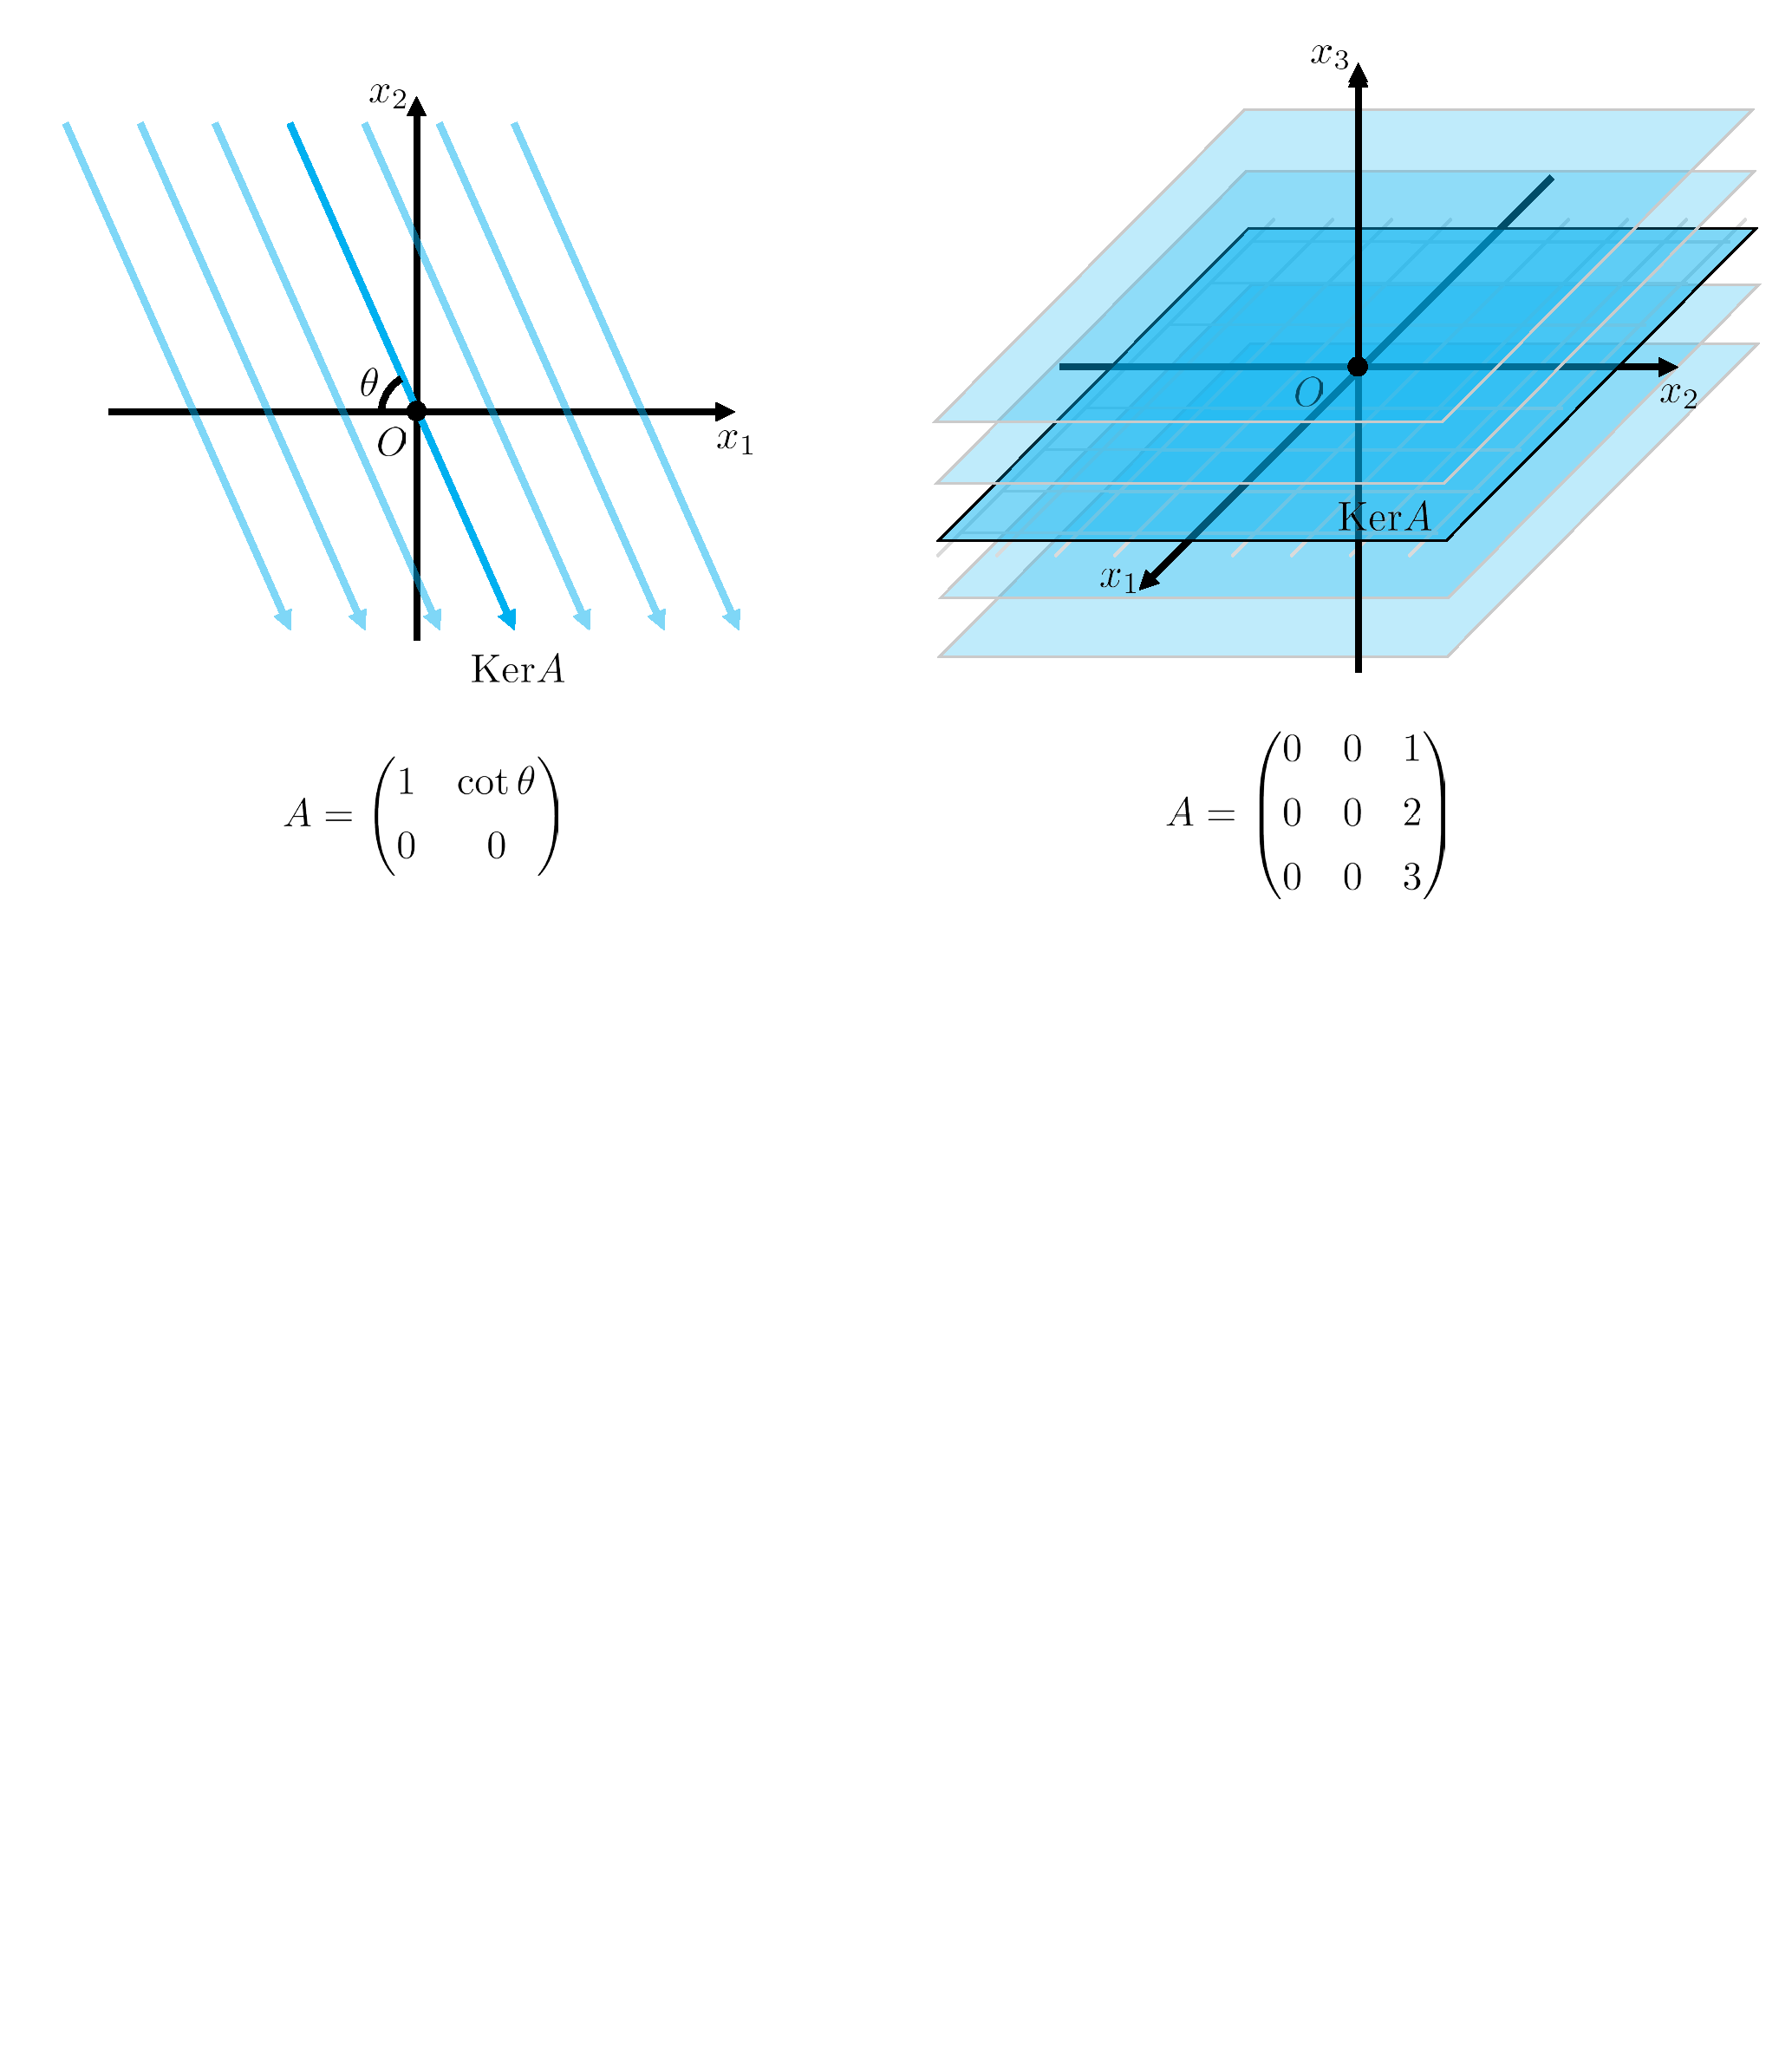
\includegraphics[trim=0 22cm 0 0, clip, width=1\textwidth]{fig/fig_x+KerA.pdf}
    \caption{线性方程组解集的结构}
    \label{fig:xKerA}
\end{figure}

\subsubsection{*再论维数公式：商集}


把上述结论放到线性映射的语境下讨论.
设$A$是$\mathbb{K}^n \to \mathbb{K}^m$的线性映射.
对任意的$\bm{\beta} \in \operatorname{Im}A \subset \mathbb{K}^m$，
$\bm{\beta}$的原像集都可表示为$\bm{\gamma} + \operatorname{Ker}A$，
其中$\bm{\gamma}$是$\bm{\beta}$在$A$下的任意一个原像.

现在固定$A$不变（因为$A$是我们的研究对象），
而允许$\bm{\beta}$变动，
这样就有一系列线性方程组$A \bm{x} = \bm{\beta}$.
由映射的性质，
当$\bm{\beta}_1 \ne \bm{\beta}_2$时，
它们不可能有公共的原像，
即$A \bm{x} = \bm{\beta}_1$与$A \bm{x} = \bm{\beta}_2$没有公共解.
另一方面，
对任意$\bm{x}_0 \in \mathbb{K}^n$，
它都有$A$中的像，
即总存在$\bm{\beta} \in \operatorname{Im}A$使得$A \bm{x}_0 = \bm{\beta}$.
于是，
$\mathbb{K}^n \to \mathbb{K}^m$的线性映射$A$能诱导出$\mathbb{K}^n$上的一个等价关系
“$\sim$”，
规定为：
\begin{eq1}
    \bm{x}_1 \sim \bm{x}_2
    ~ \Longleftrightarrow~  
    A\bm{x_1} = A\bm{x_2}
    ~ \Longleftrightarrow~ 
    \bm{x}_1 - \bm{x}_2 \in \operatorname{Ker}A
    \end{eq1}

即：$\mathbb{K}^n$中的两个向量等价当且仅当它们在$A$下的像相同，
又当且仅当它们属于同一个线性方程组$A \bm{x} = \bm{\beta}$的解集.
当$\bm{\beta}$取遍$\operatorname{Im}A$时，
线性方程组的解集$A \bm{x} = \bm{\beta}$的解集就是这个等价关系下的各个等价类.
每个等价类都可以表示成$\bm{x} + \operatorname{Ker}A$的形式.
这里重申一下这个记号的意思：
\begin{eq1}
    \bm{x} + \operatorname{Ker}A = \{ \bm{x} + \bm{x}_0  ~|~ \bm{x}_0 \in  \operatorname{Ker}A\}
\end{eq1}

从这个表达形式看出，
每个等价类都是子空间$\operatorname{Ker}A$按向量$\bm{x}$平移所得到的.
这些等价类又称为$\operatorname{Ker}A$的\textbf{陪集}.


为了从$A$诱导的等价关系得到维数公式，
需要介绍一个关于等价关系的新概念：

\clearpage

\textbf{4.~~商集}

\textbf{定义（商集）}~~
\textit{设集合$S$上有等价关系$\sim$，
那么$\sim$确定的所有等价类组成的集合称为\textbf{商集}，记作$S / \sim$.}

\textit{例7：在一个学期的所有日子中，“星期几”是一个等价关系.
于是一个学期的所有日子有一个商集$\{ \text{星期一},\text{星期二}, \cdots , \text{星期日} \}$.}

\textit{例8：奇偶等价下的商集是$\mathbb{Z}_2 = \{ \text{奇数}, \text{偶数} \}$.
或者以代表元来记等价类，就是$\mathbb{Z}_2 = \{ \bar{0},\bar{1} \}$
我们常常这样谈论奇偶性与乘法运算的关系：奇数$\times$奇数$=$奇数，
奇数$\times$偶数$=$偶数，
偶数$\times$偶数$=$偶数.
或者以代表元的形式：$\bar{1} \times \bar{1} = \bar{1}$，$\bar{1} \times \bar{0} = \bar{0}$，$\bar{0} \times \bar{0} = \bar{0}$.
}\medskip

在日常生活中，
许多商集的概念深入人心，
以至于我们不但不区分同一等价类中元素，
甚至连等价类本身都看成一种元素了.
例如，当我说“线性代数课在星期二”时，
你可能意识不到我谈论的其实是“所有星期二的集合”.
例8简明地展示了这在数学中是如何做到的.
我们会以代表元来标记等价类.
为了区分代表元所代表的等价类与代表元本身，
可以在前者的头顶上加一杠.
因此，$\bar{0}$和$\bar{1}$分别代表全体偶数和全体奇数.
这个例子中比较漂亮的一点是，
我们可以让等价类互相进行乘法运算，
运算规则与代表元的运算一致，
且与代表元的具体选取无关.
从直觉上你会认为，
“讨论乘法运算时，
$0$和$1$头上加不加那一杠实在没什么区别.
商集的概念只是在为“奇数 $\times$ 奇数”这种写法的合理性做背书而已.”
这表明你对奇偶性的熟悉程度已经像吃饭喝水一样了.
如果今后学习别的商集时也能做到这样，
那就说明理解得非常好了.

读者可能有疑问：“商集”究竟是如何得名的，
它与除法有什么关联吗？
在小学时，我们会把两个数$a$和$b$做除法的结果称为它们的“商”，
用$a / b$表示.
它可以作为如下应用题的答案：\medskip

\textit{老师端来若干个盒子，每个盒子里装有$b$块蛋糕. 
将这些蛋糕全部分发之后，全班$a$个小朋友每人都拿到$1$块蛋糕.
问共有多少个盒子？}
\medskip

鉴于读者早已小学毕业，
无需多解释“商”在这道题中反映的数量关系.
其实，
任何等价关系都可以如是看待：
某个集合中的全部元素就好比总共$a$块蛋糕，
一个个等价类就好比一个个装着$b$块蛋糕的盒子.
我们只需事先知道每个等价类中的集合个数都一样（每个盒子里蛋糕数量相同），
就能计算出共有多少个等价类（盒子的数量）.
\medskip

回到刚才的话题.
根据定义，
$\operatorname{Ker}A$的所有陪集构成的集合即是$\mathbb{K}^n$在该等价关系下的商集，
记作$\mathbb{K}^n / \operatorname{Ker}A$.
为了方便，
可以把$\bm{x} + \operatorname{Ker}A$记作$\overline{\bm{x}}$，
从而$\mathbb{K}^n / \operatorname{Ker}A = \{ \overline{\bm{x}}~|~x \in \mathbb{K}^n \}$.

现在在向量空间中，
向量就好比蛋糕，
陪集就好比盒子，
维数公式就反映了其中商的数量关系.
这里仅对此给出一个不甚严谨的解释：
从直观上，
每个陪集都是由$\operatorname{Ker}A$平移得到的，
因此每个陪集的元素“数量”应该“一样多”.
又因为每个$\operatorname{Im}A$中的元素$\bm{\beta}$都唯一确定一个陪集（即$A\bm{x} = \bm{\beta}$的解集）.
因此认为陪集的“数量”与
$\operatorname{Im}A$中的元素“数量”是“一样多”的.
因此我们有如下的商的数量关系：
\begin{eq1}
    \text{整个}\mathbb{K}^n\text{中的元素“数量”}
    &=
    \text{任意一个陪集中的元素“数量”}
    \times~
    \text{陪集的“数量”}\\[6pt]
    &= \operatorname{Ker}A~\text{中的元素“数量”}
    \times~ \operatorname{Im}A~\text{中的元素“数量”}\end{eq1}


上述公式看似美好，
但因为涉及无限集，
很难真正说清楚“元素数量”究竟有多少.
权且把它当作是对有限集情形的一种不合法的暴力推广.
不过，
如果利用向量空间中的维数概念改写此公式，
就能避开这个问题.


\begin{figure}[H] 
    \centering
    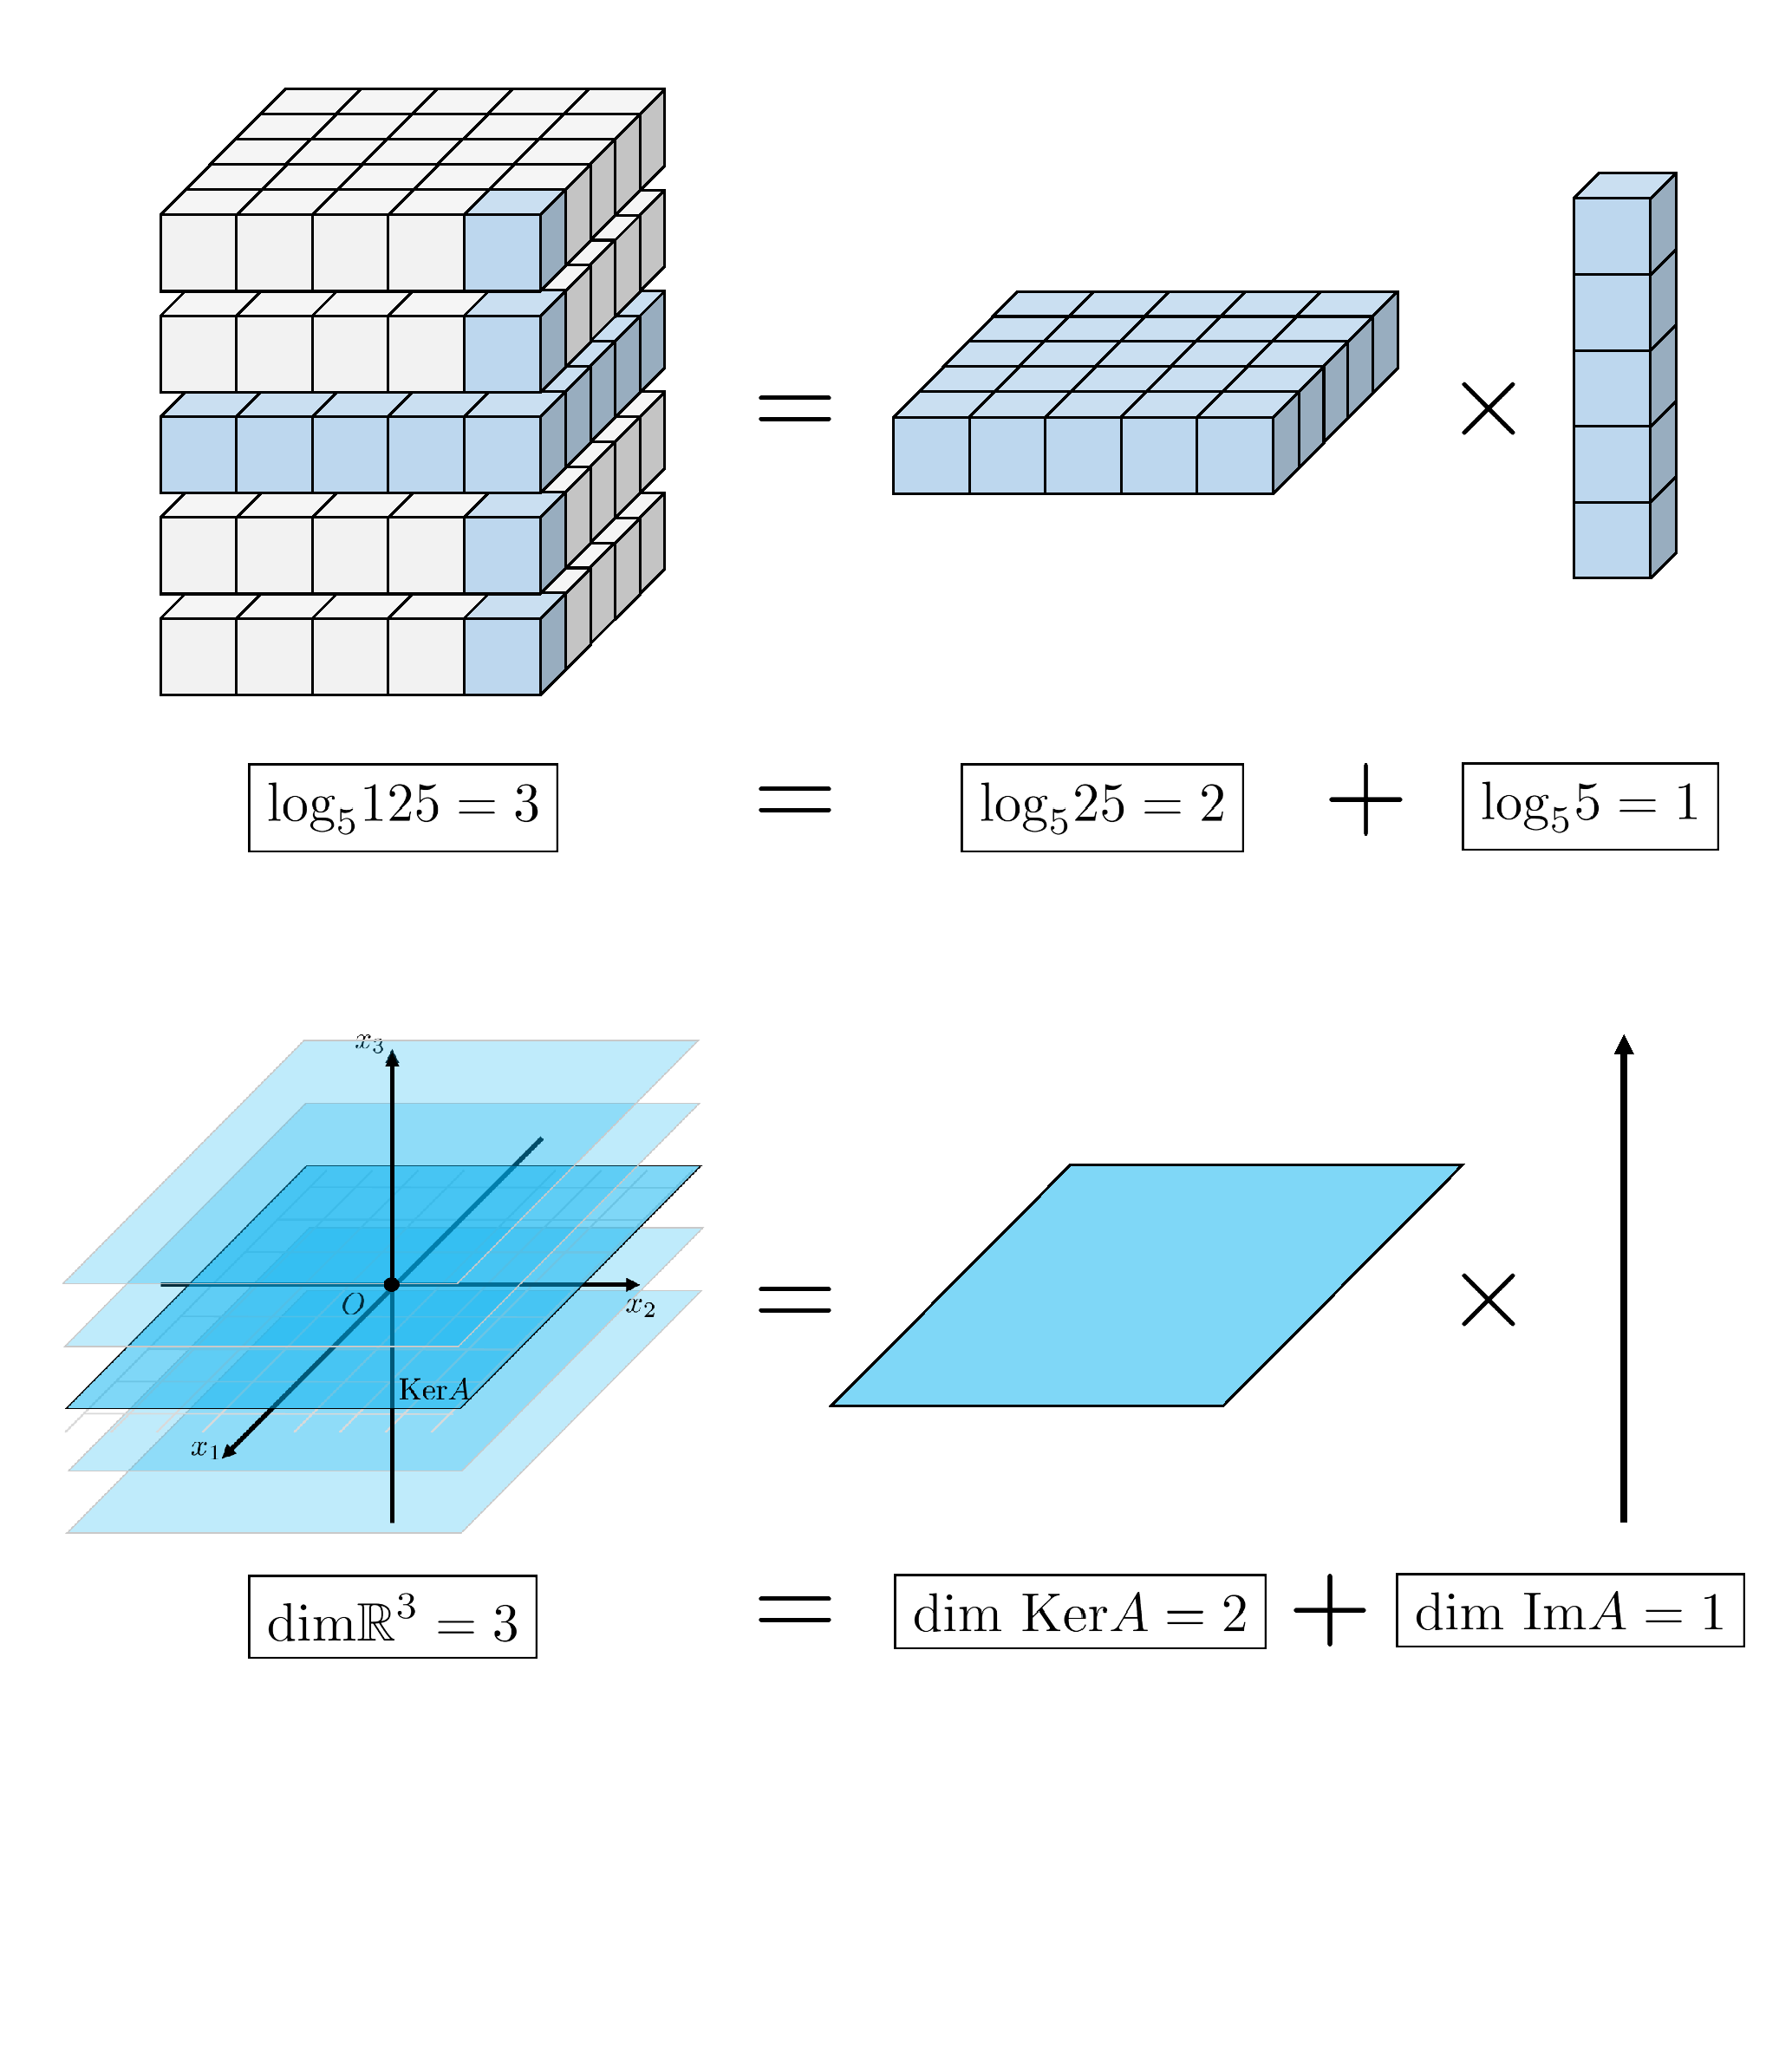
\includegraphics[trim=0 5cm 0 0, clip, width=1\textwidth]{fig/fig_logdim.pdf}
    \caption{维数公式与有限集商关系的类比}
    \label{fig:logdim}
\end{figure}
\bigskip

根据直觉，
维数应当以指数的形式计入“元素数量”中.
图\ref{fig:logdim}展示了这样想的原因.
考虑一个有限情形：
$125$个小方块拼成了一个$5 \times 5 \times 5$的大方块.
小方块的总数$125$等于每一层的小方块数$25$乘以层数$5$，
这是一个以“层”为等价类的商关系.
在这个例子中，
我们会认为小方块的堆积是在$3$个维度上进行的.
每一层的$25$个小方块是以$2$维平面的形式铺展排列，
而$5$个层的竖直堆叠又增加了$1$个维度.
在这里，
所谓维度，
可以定义成以$5$为底的对数.
原来的乘法算式改写为对数应是加法算式.
以此类比，
容易理解维数公式：
\begin{eq1}
    n = \dim\operatorname{Ker}A + \dim\operatorname{Im}A
\end{eq1}

它的意思就是，
把整个空间$\mathbb{K}^n$看成$\operatorname{Ker}A$堆叠而成.
那么，$\mathbb{K}^n$的维数应等于
$\operatorname{Ker}A$的维数加上$\operatorname{Ker}A$的堆叠所增加的维数.
更能反映上述关系的写法或许是：
\begin{eq1}
    n = \dim\operatorname{Ker}A + \dim\mathbb{K}^n / \operatorname{Ker}A
\end{eq1}

在学习了线性空间的知识以后，
我们将有能力把这一想法以严谨的数学证明的形式叙述出来.
现阶段，
重要的是获得一个正确看待线性方程组的视角.


\medskip

\subsection{习题}

\begin{example}
    $a$为何值时，
    下述线性方程组有解？
    有解时，求出所有的解.
    \begin{eq1}
        \begin{cases}
        x_1 + x_2 + x_3 + x_4 = -7 \\[2pt]
        x_1 + 3x_3 - x_4 = 8 \\[2pt]
        x_1 + 2x_2 - x_3 + x_4 = 2a + 2 \\[2pt]
        3x_1 + 3x_2 + 3x_3 + 2x_4 = -11 \\[2pt]
        2x_1 + 2x_2 + 2x_3 + x_4 = 2a
        \end{cases} \end{eq1}
\end{example}
\smallskip
\begin{solution}
    对增广矩阵用初等行变换化简的结果为：
    \begin{eq1}
        \left ( \begin{array}{cccc:c}
            1 & 1 & 1 & 1 & -7 \\[2pt]
            0 & 1 & -2 & -2 & -15 \\[2pt]
            0 & 0 & 0 & 1 & -a-12 \\[2pt]
            0 & 0 & 0 & 0 & a+2 \\[2pt]
            0 & 0 & 0 & 0 & 0
        \end{array} \right ) \end{eq1}

    方程组有解当且仅当$a=-2$.
    此时增广矩阵为：
    \begin{eq1}
        \left ( \begin{array}{cccc:c}
            1 & 1 & 1 & 1 & -7 \\[2pt]
            0 & 1 & -2 & -2 & -15 \\[2pt]
            0 & 0 & 0 & 1 & -10 \\[2pt]
            0 & 0 & 0 & 0 & 0 \\[2pt]
            0 & 0 & 0 & 0 & 0
        \end{array} \right ) \end{eq1}

    主元在第$1,2,4$列.
    取$x_3$为自由未知量.
    方程组的解可以表示为：
    \begin{eq1}
        \begin{cases}
            x_1 = -3x_3 - 2 \\[2pt]
            x_2 = 2x_3 + 5 \\[2pt]
            x_4 = -10
        \end{cases} \end{eq1}

    或者，先取自由未知量$x_3 = 1$，
    得到方程组的一个特解：
    \begin{eq1}
        \bm{\gamma} = 
        \begin{pmatrix}
            -5 \\[2pt] 7 \\[2pt] 1 \\[2pt] -10
        \end{pmatrix} \end{eq1}

    仍然取自由未知量$x_3 = 1$，
    代入相应的齐次线性方程组中，
    得到基础解系：
    \begin{eq1}
        \bm{\eta}_1 = 
        \begin{pmatrix}
            -3 \\[2pt] 2 \\[2pt] 1 \\[2pt] 0
        \end{pmatrix} \end{eq1}
    
    于是解集为$U = \{ \bm{\gamma} + c \bm{\eta}_1 ~|~ c \in \mathbb{K} \}$. \qed 
\end{solution}
\smallskip
\begin{example}
    已知向量
    \begin{eq1}
    \bm{\alpha}_1 = 
    \begin{pmatrix}
    1 \\[2pt]
    2 \\[2pt]
    4 \\[2pt]
    3
    \end{pmatrix},
    \quad
    \bm{\alpha}_2 = 
    \begin{pmatrix}
    1 \\[2pt]
    -1 \\[2pt]
    -6 \\[2pt]
    6
    \end{pmatrix},
    \quad
    \bm{\alpha}_3 = 
    \begin{pmatrix}
    -2 \\[2pt]
    -1 \\[2pt]
    2 \\[2pt]
    -9
    \end{pmatrix},
    \quad
    \bm{\alpha}_4 = 
    \begin{pmatrix}
    1 \\[2pt]
    1 \\[2pt]
    -2 \\[2pt]
    7
    \end{pmatrix},
    \quad
    \bm{\beta} = 
    \begin{pmatrix}
    4 \\[2pt]
    2 \\[2pt]
    4 \\[2pt]
    a
    \end{pmatrix},
    \end{eq1}

    (1)~~求线性子空间 \( W = \langle \bm{\alpha}_1, \bm{\alpha}_2, \bm{\alpha}_3, \bm{\alpha}_4 \rangle \) 的维数与一个基；

    (1*)~~求矩阵$A = (\bm{\alpha}_1, \bm{\alpha}_2, \bm{\alpha}_3, \bm{\alpha}_4) $的秩与它的一个极大线性无关组.

    (2)~~求 \( a \) 的值，使得 \( \bm{\beta} \in W \)，并求 \(\bm{ \beta} \) 在(1)所选基下的坐标.
\end{example}
\smallskip
\begin{remark}
    这里将(1)和(1*)放在一起比较.
    这两问实质上没有任何区别，
    做法和答案都相同.
    最方便的是用初等行变换化成阶梯形矩阵，然后寻找主元所在列.
    第(2)问实质上是解线性方程组.
\end{remark}
\smallskip
\begin{solution}
    
    (1)/(1*)~~
    矩阵$A$用初等行变换化简的结果是：
    \begin{eq1}
        \begin{pmatrix}
            1 & 1 & -2 & 1 \\[2pt]
            0 & -3 & 3 & -1 \\[2pt]
            0 & 0 & 0 & 1 \\[2pt]
            0 & 0 & 0 & 0 
        \end{pmatrix} \end{eq1}

    主元在第$1,2,4$列.
     故$W$的维数/矩阵$A$的秩为$3$.
     $W$的一组基/矩阵$A$的一个极大线性无关组是$\{ \bm{\alpha}_1 , \bm{\alpha}_2 , \bm{\alpha}_4  \}$. \medskip

     (2)~~解方程组$x_1 \bm{\alpha}_1 + x_2 \bm{\alpha}_2 + x_4 \bm{\alpha}_4  = \bm{\beta}$.
     得到唯一解$\bm{x} = (4,3,-3)$就是$\bm{\beta}$在(1)所选基下的坐标.  \qed \par
\end{solution}
\smallskip
\begin{example}
    已知向量组(I):
        \begin{eq1}
    \bm{\alpha}_1 = 
    \begin{pmatrix}
    1 \\[2pt]
    2 \\[2pt]
    0 \\[2pt]
    1
    \end{pmatrix},
    \quad
    \bm{\alpha}_2 = 
    \begin{pmatrix}
    2 \\[2pt]
    1 \\[2pt]
    1 \\[2pt]
    0
    \end{pmatrix},
    \quad
    \bm{\alpha}_3 = 
    \begin{pmatrix}
    3 \\[2pt]
    3 \\[2pt]
    1 \\[2pt]
    1
    \end{pmatrix},
    \quad
    \bm{\alpha}_4 = 
    \begin{pmatrix}
    0 \\[2pt]
    1 \\[2pt]
    -1 \\[2pt]
    1
    \end{pmatrix}
    \end{eq1}

    向量组(II):
    \begin{eq1}
    \bm{\beta}_1 = 
    \begin{pmatrix}
    4 \\[2pt]
    5 \\[2pt]
    1 \\[2pt]
    2
    \end{pmatrix},
    \quad
    \bm{\beta}_2 = 
    \begin{pmatrix}
    1 \\[2pt]
    3 \\[2pt]
    -1 \\[2pt]
    2
    \end{pmatrix},
    \quad
    \bm{\beta}_3 = 
    \begin{pmatrix}
    5 \\[2pt]
    6 \\[2pt]
    2 \\[2pt]
    2
    \end{pmatrix}
    \end{eq1}

    问这两个向量组是否等价？
\end{example}
\smallskip
\begin{remark}
    无需验证(I)和(II)能相互线性表示.
    只需将(I)和(II)分别拼成矩阵$A$和$B$，
    验证矩阵$A,B,(A,B)$的秩相同.
\end{remark}
\smallskip
\begin{solution}
    容易验证$A$和$B$的秩都是$3$.
    矩阵$(A,B)$用初等行变换化简的结果是：
    \begin{eq1}
        \begin{pmatrix}
            1 & 2 & 3 & 0 & 4 & 1 & 5 \\[2pt]
            0 & 1 & 1 & -1 & 1 & -1 & 2 \\[2pt]
            0 & 0 & 0 & 1 & 0 & 1 & -1 \\[2pt]
            0 & 0 & 0 & 0 & 0 & 0 & 0
        \end{pmatrix} \end{eq1}
    
    它的秩也是$3$.
    故向量组(I)和(II)等价. \qed \par
\end{solution}
\smallskip
\begin{example}
    讨论以下$n$阶矩阵的秩：
    \begin{eq1}
        A_n = 
        \begin{pmatrix}
            1+x & 1 & 1 & \cdots & 1 & 1  \\[2pt]
            1 & 1+x & 1 & \cdots & 1 & 1  \\[2pt]
            1 & 1 & 1+x & \cdots & 1 & 1  \\[2pt]
            \vdots & \vdots & \vdots & \ddots & \vdots & \vdots \\[2pt]
            1 & 1 & 1 & \cdots & 1+x & 1  \\[2pt]
            1 & 1 & 1 & \cdots & 1 & 1+x 
        \end{pmatrix} \end{eq1}
\end{example}
\smallskip
\begin{solution}
    把$A_n$的第一行减到其余所有行上：
    \begin{eq1}
        \begin{pmatrix}
    1+x & 1 & 1 & \cdots & 1 \\[2pt]
    -x  & x & 0 & \cdots & 0 \\[2pt]
    -x  & 0 & x & \cdots & 0 \\[2pt]
    \vdots & \vdots & \vdots & \ddots & \vdots\\[2pt]
    -x  & 0 & 0 & \cdots & x
    \end{pmatrix}\end{eq1}

    再把除第1列之外的所有列加到第1列上：
    \begin{eq1}
        \begin{pmatrix}
        n+x & 1 & 1 & \cdots & 1 \\[2pt]
        0  & x & 0 & \cdots & 0 \\[2pt]
        0  & 0 & x & \cdots & 0 \\[2pt]
        \vdots & \vdots & \vdots & \ddots & \vdots\\[2pt]
        0  & 0 & 0 & \cdots & x
        \end{pmatrix}\end{eq1}

    (i)~若$x=0$，
    $\mathrm{rank}(A_n) = 1$.

    (ii)~若$x=-n$，
    $\mathrm{rank}(A_n) = n-1$.

    (iii)~若$x\ne 0$且$x \ne -n$，
    $\mathrm{rank}(A_n) = n$.
    \qed
\end{solution}

\bigskip

\begin{example}
    设有齐次线性方程组：
    \begin{eq1}
        \begin{cases}
            (1+a)x_1 + x_2 + \cdots + x_n = 0 \\[2pt]
            2x_1 + (2+a)x_2 + \cdots + 2x_n = 0 \\[2pt]
            \vdots \\[2pt]
            nx_1 + nx_2 + \cdots + (n+a)x_n = 0 
        \end{cases}\end{eq1}

    其中$n \ge 2$.
    试问$a$取何值时，该方程组有非零解？
    并求出其通解.
\end{example}
\smallskip
\begin{solution}
    系数矩阵：
    \begin{eq1}
        \begin{pmatrix}
        1+a & 1 & 1 & \cdots & 1 \\[2pt]
        2  & 2+a & 2 & \cdots & 2 \\[2pt]
        3  & 3 & 3+a & \cdots & 3 \\[2pt]
        \vdots & \vdots & \vdots & \ddots & \vdots\\[2pt]
        n  & n & n & \cdots & n+a
        \end{pmatrix}\end{eq1}
    
    把所有行加到第$n$行上：
    \begin{eq1}
        \begin{pmatrix}
        1+a & 1 & 1 & \cdots & 1 \\[4pt]
        2  & 2+a & 2 & \cdots & 2 \\[4pt]
        3  & 3 & 3+a & \cdots & 3 \\[4pt]
        \vdots & \vdots & \vdots & \ddots & \vdots\\[4pt]
        n-1  & n-1 & n-1 & \cdots & n-1 \\[4pt]
        \frac{n(n+1)}{2}+a & \frac{n(n+1)}{2}+a & \frac{n(n+1)}{2}+a & \cdots & \frac{n(n+1)}{2}+a 
        \end{pmatrix}\end{eq1}

    (i)~若$a = -\frac{n(n+1)}{2}$，
    则最后一行现在是零行，
    因此该方程组有非零解.

    将第$1$行的$-i$倍加到第$i$行上$(i = 2,\cdots, n-1)$，
    除掉公因数$a$：
    \begin{eq1}
        \begin{pmatrix}
        1+a & 1 & 1 & \cdots & 1 & 1 \\[2pt]
        -2  & 1 & 0 & \cdots & 0 & 0 \\[2pt]
        -3  & 0 & 1 & \cdots & 0 & 0 \\[2pt]
        \vdots & \vdots & \vdots & \ddots & \vdots & \vdots\\[2pt]
        -(n-1)  & 0 & 0 & \cdots & 1 & 0 \\[2pt]
        0 & 0 & 0 & \cdots & 0 & 0
        \end{pmatrix}\end{eq1}

    取$x_1$为自由未知量，
    代入，得到通解：
    \begin{eq1}
        \begin{cases}
            x_1 = x_1 \\[2pt]
            x_2 = 2x_1 \\[2pt]
            \cdots \\[2pt]
            x_{n-1} = (n-1)x_1 \\[2pt]
            x_n = -n^2 x_1
        \end{cases} \end{eq1}

    \medskip

    (ii)~若$a \ne -\frac{n(n+1)}{2}$，
    则最后一行除以$a + \frac{n(n+1)}{2}$，
    得到：
    \begin{eq1}
        \begin{pmatrix}
        1+a & 1 & 1 & \cdots & 1 \\[2pt]
        2  & 2+a & 2 & \cdots & 2 \\[2pt]
        3  & 3 & 3+a & \cdots & 3 \\[2pt]
        \vdots & \vdots & \vdots & \ddots & \vdots\\[2pt]
        1  & 1 & 1 & \cdots & 1
        \end{pmatrix}\end{eq1}

    把最后一行的$-i$倍加到第$i$行上$(i = 1,2,\cdots, n-1)$：
    \begin{eq1}
        \begin{pmatrix}
        a & 0 & 0 & \cdots & 0 \\[2pt]
        0  & a & 0 & \cdots & 0 \\[2pt]
        0  & 0 & a & \cdots & 0 \\[2pt]
        \vdots & \vdots & \vdots & \ddots & \vdots\\[2pt]
        1  & 1 & 1 & \cdots & 1
        \end{pmatrix}\end{eq1}

    只有当$a=0$时，
    系数矩阵不满秩，
    原方程组有非零解.
    此时秩为$n-1$，
    取$x_1, x_2,\cdots,x_{n-1}$为$n$个自由未知量，
    代入，
    得到通解：
    \begin{eq1}
        \begin{cases}
            x_1 = x_1 \\[2pt]
            x_2 = x_2 \\[2pt]
            \cdots \\[2pt]
            x_{n-1} = x_{n-1} \\[2pt]
            x_n = -x_1 - x_2 -\cdots - x_{n-1}
        \end{cases} \end{eq1} 
    \qed

\end{solution}
\smallskip
\begin{example}
    设$\bm{\alpha}_1, \bm{\alpha}_2 , \cdots , \bm{\alpha}_s$是一组线性无关的向量.
    问$\bm{\alpha}_1+ \bm{\alpha}_2, \bm{\alpha}_2+ \bm{\alpha}_3, \cdots ,\bm{\alpha}_{s-1}+ \bm{\alpha}_s , \bm{\alpha}_s+ \bm{\alpha}_1$
    是否线性无关？请证明之.
\end{example}
\smallskip
\begin{pf}
    考虑线性方程组
    $x_1(\alpha_1+\alpha_2)+
    x_2(\alpha_2+\alpha_3)+
    \cdots 
    +x_s(\alpha_s+\alpha_1)=0$.

    重新整理得到：
    $(x_1+x_s)\alpha_1
    +(x_1+x_2)\alpha_2
    +(x_2+x_3)\alpha_3
    +\cdots
    +(x_{s-1}+x_s)\alpha_s=0$.
    
    由于$\alpha_1,\dots,\alpha_s$线性无关，故各系数必为零：
    \begin{eq1}
        \begin{cases}
        x_1~~~~~~~~~~~~~~~~~~~~~~~~~~+x_s&=0\\[2pt]
        x_1+x_2&=0\\[2pt]
        ~~~~~~~x_2+x_3&=0\\[2pt]
        ~~~~~~~~~~~~~~~~\ddots \\[2pt]
        ~~~~~~~~~~~~~~~~~~~~~~~x_{s-1}+x_s&=0
        \end{cases} \end{eq1}

    这给出了一个关于$x_1,x_2 ,\cdots, x_s$的线性方程组，
    其系数矩阵为：
    \begin{eq1}
        \begin{pmatrix}
        1 & 0 & 0 & \cdots & 1 \\[2pt]
        1  & 1 & 0 & \cdots & 0 \\[2pt]
        0  & 1 & 1 & \cdots & 0 \\[2pt]
        \vdots & \vdots & \vdots & \ddots & \vdots\\[2pt]
        0  & 0 & 0 & \cdots & 1
        \end{pmatrix}\end{eq1}

    将第$i$行$(i = 2,3,\cdots,s)$的$(-1)^{s-i+1}$倍加到第1行上.
    
    (i)~若$s$是偶数，
    则第1行变为零行，
    系数矩阵不满秩，
    方程组有非零解，
    故向量组线性相关.

    (ii)~若$s$是奇数，
    则矩阵化为下三角且对角元都非零，
    系数矩阵满秩，
    方程组只有零解，
    故向量组线性无关.

\end{pf}

\bigskip

\begin{example}
    设向量组$\bm{\alpha}_1, \bm{\alpha}_2 , \cdots , \bm{\alpha}_s$线性无关，
    并且可由向量组$\bm{\beta}_1, \bm{\beta}_2 , \cdots , \bm{\beta}_t$线性表示.
    证明：必存在某个向量$\bm{\beta}_j (j = 1,2,\cdots , t)$使得向量组
    $\bm{\beta}_j, \bm{\alpha}_2 , \cdots , \bm{\alpha}_s$线性无关.
\end{example}
\smallskip
\begin{remark}
    本题直接从向量组的角度和从子空间的角度出发都可以证明.
\end{remark}
\smallskip
\begin{solution}(1. 向量组方法)
    取$\{ \bm{\beta}_1, \bm{\beta}_2 , \cdots , \bm{\beta}_t \}$
    的一个极大线性无关组$\{ \bm{\beta}_{j_1}, \bm{\beta}_{j_2} , \cdots , \bm{\beta}_{j_r} \}$，
    它也能线性表示向量组$\{\bm{\alpha}_1, \bm{\alpha}_2 , \cdots , \bm{\alpha}_s \}$.
    由命题2.1.7，
    $\{ \bm{\beta}_{j_1}, \bm{\beta}_{j_2} , \cdots , \bm{\beta}_{j_r} \}$，
    与$\{\bm{\alpha}_1, \bm{\alpha}_2 , \cdots , \bm{\alpha}_s \}$
    等价，
    从而后者也能线性表示前者，
    即任意的$\bm{\beta}_{ji}$可以表示为
    $\bm{\beta}_{ji} = c_1\bm{\alpha}_1 + c_2\bm{\alpha}_2 + \cdots + c_s\bm{\alpha}_s$.

    用反证法.
    假设对任意的$\bm{\beta}_j$，
    向量组$\{ \bm{\beta}_j ,\bm{\alpha}_2 , \cdots,  \bm{\alpha}_s \}$线性相关.
    则$\{ \bm{\beta}_{ji} ,  \bm{\alpha}_2 , \cdots, \bm{\alpha}_s\}$一定线性相关.
    但这个向量组与$\{\bm{\alpha}_1, \bm{\alpha}_2 , \cdots , \bm{\alpha}_s \}$等价，
    它是线性无关的，
    矛盾.
    \qed
\end{solution}
\begin{solution}(2.子空间方法)
    反证法.
    假设对任意的$\bm{\beta}_j$，
    向量组$\{ \bm{\beta}_j ,\bm{\alpha}_2 , \cdots,  \bm{\alpha}_s \}$线性相关.
    因为$\{\bm{\alpha}_1, \bm{\alpha}_2 , \cdots,  \bm{\alpha}_s \}$线性无关，
    其部分组$\{ \bm{\alpha}_2 , \cdots,  \bm{\alpha}_s \}$也线性无关.
    所以对任意的$j = 1,2,\cdots, t$，
    有$\bm{\beta}_j \in \langle \bm{\alpha}_2 , \cdots,  \bm{\alpha}_s \rangle$（利用例1.7的结论），
    因此：
    \begin{eq1}
        \langle \bm{\beta}_1, \bm{\beta}_2 , \cdots , \bm{\beta}_t \rangle 
        \subset \langle \bm{\alpha}_2 , \cdots,  \bm{\alpha}_s \rangle
        \subsetneq \langle \bm{\alpha}_1 , \bm{\alpha}_2 , \cdots,  \bm{\alpha}_s \rangle
    \end{eq1}

    但是题设表明：
    \begin{eq1}
        \langle \bm{\alpha}_1, \bm{\alpha}_2 , \cdots , \bm{\alpha}_s \rangle
        \subset \langle \bm{\beta}_1, \bm{\beta}_2 , \cdots , \bm{\beta}_t \rangle
    \end{eq1}
    
    矛盾. \qed    
\end{solution}



\bigskip

\begin{example}
    设 $\mathbb{K}$ 为一个数域，$n$ 为大于 $1$ 的正整数.
    已知 $\bm{\gamma} \in \mathbb{K}^n$为$n$个未知量的非齐次线性方程组
    $A \bm{x} = \bm{\beta}$ 的一个解，
    并且 $\bm{\eta}_1, \bm{\eta}_2, \dots, \bm{\eta}_{n-r} \in \mathbb{K}^n$
    （$r$ 为大于 $1$ 小于 $n$ 的正整数）
    为齐次线性方程组$A\bm{x} = \bm{0}$的基础解系.
    求证：

    (1)~向量组 $\bm{\gamma},\ \bm{\gamma}+\bm{\eta}_1,\ \bm{\gamma}+\bm{\eta}_2,\ \dots,\ \bm{\gamma}+\bm{\eta}_{n-r}$ 线性无关.

    (2)~方程组 $A \bm{x} = \bm{\beta}$
    的任一个解都可以被向量组$\bm{\gamma},\ \bm{\gamma}+\bm{\eta}_1,\ \bm{\gamma}+\bm{\eta}_2,\ \dots,\ \bm{\gamma}+\bm{\eta}_{n-r}$线性表出.
    线性表出的系数满足什么规律？
\end{example}
\smallskip
\begin{remark}
    第(2)问在$n=2$时的特殊情形即是平面向量共线定理：
    设$\bm{\eta}_1$和$\bm{\eta}_2$是$\mathbb{R}^2$上某条直线上的两个不同的点（非原点），
    则$\bm{x}$落在这条直线上当且仅当$\bm{x} = k_1 \bm{\eta}_1 + k_2 \bm{\eta}_2$，
    其中$k_1 + k_2 = 1$.
    类似地有空间向量共面定理.
\end{remark}
\smallskip
\begin{pf}
    (1)~
    注意向量组中的每个向量都有含有$\bm{\gamma}$.
    将它们消去，
    可以得到一个更简单而且等价的向量组$\bm{\gamma}, \bm{\eta}_1 , \bm{\eta}_2 ,\dots , \bm{\eta}_{n-r}$.
    只需去证它是线性无关的.

    用反证法，
    假设它是线性相关的，
    则由于基础解系$\bm{\eta}_1, \bm{\eta}_2, \dots, \bm{\eta}_{n-r}$是线性无关的，
    根据例1.7的结论，
    $\bm{\gamma} \in \langle \bm{\eta}_1, \bm{\eta}_2, \dots, \bm{\eta}_{n-r} \rangle = \operatorname{Ker}A$，
    即$A\bm{\gamma} = \bm{0}$，
    矛盾.

    \medskip

    (2)~任取$A\bm{x} = \bm{\beta}$的一个解$\bm{x}$，
    则$\bm{x} - \bm{\gamma}$是齐次方程组$A\bm{x} = \bm{0}$的一个解.
    因此可由基础解系线性表出：
    \begin{eq1}
        \bm{x} - \bm{\gamma} 
        = k_1 \bm{\eta}_1+ k_2 \bm{\eta}_2+\dots+ k_{n-r} \bm{\eta}_{n-r}
    \end{eq1}

    于是有：\bigskip
    \begin{eq1}
        \bm{x}
        &= k_1 \bm{\eta}_1+ k_2 \bm{\eta}_2+\dots+ k_{n-r} \bm{\eta}_{n-r} +  \bm{\gamma}\\[4pt]
        &= k_1 (\bm{\eta}_1 + \bm{\gamma})
        + k_2 (\bm{\eta}_2 + \bm{\gamma})
        + \cdots 
        + k_{n-r} (\bm{\eta}_{n-r} + \bm{\gamma}) + (1-k_1 - k_2 - \cdots - k_{n-r})\bm{\gamma} \end{eq1}

    其中各系数$k_1, k_2 , \cdots, k_{n-r}, 1-k_1 - k_2 - \cdots - k_{n-r}$
    总和为$1$. 
\end{pf}

\bigskip

\begin{example}
    有三张$\mathbb{R}^3$中的平面$a_{i}x + b_{i}y + c_i z = d_i~(i=1,2,3)$.
    其中，有$2$张平面平行，
    第$3$张平面与它们相交.
    若将这$3$个平面方程组成一个线性方程组，
    其系数矩阵和增广矩阵的秩分别是？
\end{example}
\smallskip
\begin{solution}
    系数矩阵的第$i$个行向量$(a_i,b_i,c_i)$是对应平面的法向量.
    现在有$2$张平面平行，
    有$2$张平面平行，
    第$3$张平面与它们相交，
    表明有$2$个行向量是共线的，
    第$3$个行向量与之不共线，
    即系数矩阵的秩为$2$.

    线性方程组的解集可以看成三张平面的公共点集.
    因为有两张平面平行，
    解集为空.
    根据线性方程组有解的判定定理，
    增广矩阵的秩应该大于$2$.
    而增广矩阵有$3$行，秩至多是$3$，
    因此增广矩阵的秩就是$3$.\qed
\end{solution}